% =====================================================================
%  ASM Track — Rapport de Projet de Fin d'Études
%  Compilation :  latexmk -pdf main.tex        (ou pdflatex ×3 + biber)
%
%  Cible : ~140 pages  =  12 liminaires + 118 corps + 10 annexes/biblio.
%  Le budget de pages de chaque chapitre est rappelé en tête de son fichier.
% =====================================================================
\documentclass[12pt,a4paper,oneside]{report}

% =====================================================================
%  Préambule — mise en forme, packages, commandes maison.
%  Rien de spécifique au contenu ici : le texte vit dans chapters/.
% =====================================================================

% ---------- Langue et écriture ----------
%
%  COMPILER AVEC XeLaTeX  (xelatex main.tex), pas pdflatex.
%
%  Le modèle de l'institut impose un résumé en arabe sur la dernière page. pdfLaTeX ne sait pas
%  composer l'arabe : il ne gère ni le sens droite-à-gauche ni les ligatures contextuelles. On passe
%  donc par XeTeX, fontspec et polyglossia, qui lisent directement les polices système. C'est aussi
%  pourquoi babel, inputenc et fontenc ont disparu : ils sont incompatibles avec polyglossia et
%  inutiles sous XeTeX, dont l'entrée est nativement UTF-8.
\usepackage{fontspec}
\usepackage{polyglossia}
\setmainlanguage{french}
\setotherlanguage{arabic}
% Times New Roman, corps 12 : imposé par le guide de rédaction de l'institut (règle 1).
\setmainfont{Times New Roman}
\newfontfamily\arabicfont[Script=Arabic]{Amiri}  % naskh académique, fourni par MiKTeX
\usepackage{csquotes}          % requis par biblatex pour les guillemets

% ---------- Typographie ----------
\usepackage{microtype}
\usepackage{setspace}
\onehalfspacing                % interligne 1,5 — attendu par la plupart des jurys
\usepackage{parskip}

% ---------- Géométrie ----------
% Largeur et hauteur de texte imposées par le guide de rédaction (règle 3) : 160 × 250 mm sur A4
% (210 × 297 mm). Ne pas fixer les marges directement : sans elles, geometry centre le bloc de
% texte pour obtenir cette largeur et cette hauteur exactement, ce qui est le résultat demandé.
% bindingoffset décale le bloc vers la droite pour la reliure collée, sans toucher à sa largeur :
% le pli en avale environ 5 mm, qui seraient sinon pris sur la marge de gauche.
% headheight : fancyhdr reclame 14.5pt et n'en recoit que 12 par defaut, ce qu'il signale a chaque
% page. L'option est passee a geometry plutot que fixee apres coup : geometry ajuste alors la marge
% haute et laisse textheight a 250mm exactement, comme la regle 3 l'impose. La fixer par
% \setlength apres le chargement ferait deborder le bloc de 2.5pt vers le bas.
\usepackage[a4paper,textwidth=160mm,textheight=250mm,bindingoffset=5mm,headheight=14.5pt]{geometry}

% ---------- Figures et tableaux ----------
\usepackage{graphicx}
% Les diagrammes sont ranges par sprint depuis leur reorganisation : chaque dossier est
% declare ici, sinon \includegraphics ne trouve rien a la racine de drawio/.
\graphicspath{{figures/}{figures/logos/}{../diagrams/drawio/}{../diagrams/drawio/Sprint0/}
  {../diagrams/drawio/Sprint1/}{../diagrams/drawio/Sprint2/}{../diagrams/drawio/Sprint3/}
  {../diagrams/drawio/Sprint4/}{../diagrams/drawio/Sprint5/}{../diagrams/drawio/Architecture/}
  {../diagrams/drawio/chap9/}{../diagrams/svg/}{../docs/assets/uml/}}
% Les diagrammes UML sont reduits pour tenir dans le bloc de texte, et leurs libelles descendent
% alors sous la taille lisible. Le bloc fait 160 mm sur une page de 210 : une figure peut occuper
% 190 mm sans toucher le bord, soit 19 % de texte en plus, sans rien changer au diagramme. Le
% \makebox garde la figure centree sur le bloc et empeche LaTeX de signaler un debordement.
\newcommand{\diagramme}[2][0.45]{%
  \makebox[\textwidth][c]{\includegraphics[width=190mm,height=#1\textheight,keepaspectratio]{#2}}}
% Les deux diagrammes de sequence les plus larges restaient illisibles en portrait : reduits pour
% tenir dans 190 mm, leurs libelles descendaient sous 4 pt. Ils occupent desormais une page entiere
% en paysage, ou la largeur utile passe a 280 mm. pdflscape fait pivoter la page dans le lecteur,
% de sorte que la figure se lit sans tourner le document imprime.
\usepackage{pdflscape}
% La hauteur est la dimension contraignante pour ces deux diagrammes : en paysage, le bloc de texte
% n'en offre que 160 mm alors que la page tournee en fait 210, marges comprises. On lui en rend 15,
% ce qui laisse 10 mm sous la legende : la figure passe de 132 mm en portrait a 163, soit 24 % de
% plus. Au-dela, la legende sort de la feuille sans que LaTeX ne signale rien.
\newcommand{\diagrammepaysage}[3]{%
  \begin{landscape}
  \enlargethispage{15mm}%
  \begin{figure}[H]\centering
  \makebox[\textwidth][c]{\includegraphics[width=270mm,height=163mm,keepaspectratio]{#1}}
  \caption{#2}\label{#3}
  \end{figure}
  \end{landscape}}
\usepackage{float}
% Les figures en [H] laissaient de grands blancs : quand l'image ne tenait plus dans la place
% restante, LaTeX abandonnait le bas de la page. En [htbp] elles flottent vers le haut ou le bas de
% la page, et le texte comble. placeins/section les empeche de deriver au-dela de leur section, de
% sorte qu'une figure reste toujours dans la section qui l'annonce.
\usepackage[section]{placeins}
% placeins ne pose sa barriere qu'aux \section. Sans cette extension aux \subsection, une figure
% annoncee dans une sous-section peut deriver jusqu'a la fin de la section : le diagramme de cas
% d'utilisation du sprint 3 arrivait quatre pages apres la phrase qui l'annonce, une fois passes
% les trois tableaux de cas detailles.
\makeatletter
\AtBeginDocument{%
  \expandafter\renewcommand\expandafter\subsection\expandafter{%
    \expandafter\@fb@secFB\subsection}%
}
\makeatother
% Seuils de flottement. Par defaut LaTeX refuse qu'une figure occupe plus de 70 % du haut d'une page
% et exige 20 % de texte, ce qui reporte les grandes images et laisse des demi-pages blanches. On lui
% permet d'aller jusqu'a 92 % en haut, de n'exiger que 5 % de texte, et de remplir une page de
% flottants des 60 %, au lieu de 50.
\renewcommand{\topfraction}{0.92}
\renewcommand{\bottomfraction}{0.85}
\renewcommand{\textfraction}{0.05}
\renewcommand{\floatpagefraction}{0.60}
\setcounter{topnumber}{3}
\setcounter{bottomnumber}{2}
\setcounter{totalnumber}{5}
% Espacement autour des flottants place en [H] : la valeur par defaut de LaTeX est genereuse et
% suffisait, sur une page deja chargee, a faire basculer la figure suivante a la page d'apres en
% laissant un grand blanc. La resserrer fait tenir un couple texte + capture de plus par page.
\setlength{\intextsep}{10pt plus 2pt minus 3pt}
\setlength{\textfloatsep}{12pt plus 2pt minus 4pt}
\usepackage{caption}
\usepackage{subcaption}
\usepackage{booktabs}
\usepackage{longtable}
\usepackage{tabularx}
\usepackage{multirow}
\usepackage{array}
\usepackage[table]{xcolor}

% Colonnes de largeur fixe, alignées à gauche / centrées / à droite.
\newcolumntype{L}[1]{>{\raggedright\arraybackslash}p{#1}}
\newcolumntype{C}[1]{>{\centering\arraybackslash}p{#1}}
\newcolumntype{R}[1]{>{\raggedleft\arraybackslash}p{#1}}

% ---------- Mise en page libre (couverture, page de résumé) ----------
\usepackage{tikz}
\usetikzlibrary{calc}

% ---------- Couleurs ----------
% Les deux premières sont relevées sur la charte ISIMS (bande de couverture) : la couverture doit
% rester conforme au modèle de l'institut, ce n'est pas un choix esthétique.
\definecolor{isimsblue}{HTML}{1F6CA0}
\definecolor{isimsyellow}{HTML}{D9DE28}
\definecolor{primary}{HTML}{1B5E20}
\definecolor{accent}{HTML}{00897B}
\definecolor{codebg}{HTML}{F5F5F5}

% ---------- En-têtes ----------
\usepackage{fancyhdr}
\pagestyle{fancy}
\fancyhf{}
\fancyhead[L]{\nouppercase{\leftmark}}
\fancyhead[R]{\thepage}
\renewcommand{\headrulewidth}{0.4pt}
\fancypagestyle{plain}{\fancyhf{}\fancyfoot[C]{\thepage}\renewcommand{\headrulewidth}{0pt}}

% ---------- Titres de chapitre ----------
% Motif carré noir + numéro blanc, titre à côté, filet en dessous : observé identique dans deux
% mémoires ISIMS réels (couverture de ce document et le mémoire InvisiThreat pris comme modèle),
% sur les titres de chapitre ET les titres de section non numérotés (Dédicace, Remerciements, Table
% des matières...). C'est la convention de l'institut, pas un choix esthétique — d'où l'abandon du
% vert utilisé dans une version précédente : rien dans le modèle observé n'est en couleur.
%
% titlesec ne permet pas facilement de mettre une étiquette et un titre côte à côte à la même
% hauteur (son mode [display] les empile verticalement) ; on redéfinit donc directement les
% macros internes de la classe report, qui donnent un contrôle total sur la mise en page.
\newcommand{\chapitrebadge}[1]{%
  \tikz[baseline=-0.5ex]{\node[fill=black,text=white,font=\bfseries\Large,
    minimum width=1.2cm,minimum height=1.2cm,inner sep=0pt]{#1};}%
}
\makeatletter
% Chapitre numéroté (corps du mémoire).
\def\@makechapterhead#1{%
  \vspace*{10\p@}%
  \parindent\z@\raggedright
  \begin{minipage}[b]{2.1cm}
    % \chaptertitlename n'existe pas en LaTeX standard — c'est un alias fourni par titlesec, qui
    % n'est plus chargé ici. \@chapapp est la vraie macro du noyau (report.cls) : elle vaut
    % « Chapitre » ou « Annexe » selon qu'on est dans \appendix ou non, et suit la langue active.
    % Largeur 2,1cm : à 1,5cm, « CHAPITRE » en dépassait de 0,5cm (overfull hbox).
    \normalfont\small\bfseries\MakeUppercase{\@chapapp}\\[6pt]
    \chapitrebadge{\thechapter}
  \end{minipage}%
  \hfill
  \begin{minipage}[b]{0.70\textwidth}
    \raggedright\normalfont\Large\bfseries #1
  \end{minipage}\par\nobreak
  \vskip 10\p@
  \noindent\rule{\textwidth}{1pt}
  \vskip 24\p@
}
% Chapitre non numéroté (\chapter*{...} : Dédicace, Remerciements, Annexes...) : même filet, mais
% un carré plein sans numéro à la place du badge, comme dans le modèle.
\def\@makeschapterhead#1{%
  \vspace*{10\p@}%
  \parindent\z@\raggedright
  \tikz{\node[fill=black,minimum width=0.4cm,minimum height=1.1cm,inner sep=0pt]{};}%
  \hspace{10pt}%
  {\normalfont\Large\bfseries #1}\par\nobreak
  \vskip 10\p@
  \noindent\rule{\textwidth}{1pt}
  \vskip 24\p@
}
\makeatother

% ---------- Code source ----------
\usepackage{listings}
\lstset{
  basicstyle=\ttfamily\footnotesize,
  backgroundcolor=\color{codebg},
  keywordstyle=\color{primary}\bfseries,
  commentstyle=\color{gray}\itshape,
  stringstyle=\color{accent},
  numbers=left, numberstyle=\tiny\color{gray}, numbersep=8pt,
  breaklines=true, showstringspaces=false,
  frame=single, rulecolor=\color{gray!40},
  captionpos=b,
  % Les extraits contiennent des accents (commentaires en français).
  extendedchars=true, literate={é}{{\'e}}1 {è}{{\`e}}1 {à}{{\`a}}1 {ê}{{\^e}}1 {ç}{{\c c}}1 {û}{{\^u}}1 {ô}{{\^o}}1 {î}{{\^\i}}1
}

% ---------- Éviter un pied de page orphelin ----------
\usepackage{needspace}

% ---------- Listes ----------
\usepackage{enumitem}
\setlist{itemsep=2pt,topsep=4pt}

% ---------- Liens ----------
\usepackage[hidelinks]{hyperref}
\hypersetup{
  pdftitle={ASM Track — Rapport de Projet de Fin d'Études},
  pdfauthor={Mohamed Aziz Hadj Kacem},
  bookmarksnumbered=true
}

% ---------- Bibliographie ----------
% Le guide de rédaction (règle 4) impose un corps 10 et un style par abréviation entre crochets :
% [ROU 99] pour Paul Rouet, 1999, soit trois lettres du nom, une espace, deux chiffres de l'année.
% \bibfont est le point d'entrée officiel de biblatex pour la taille de police de la liste.
% maxalphanames=1 : l'etiquette ne retient que le premier auteur, sans quoi biblatex accole trois
% lettres de chacun (SCHSUT pour Schwaber et Sutherland). labelalphaothers vide supprime le « + »
% que le style ajoute des qu'une liste d'auteurs est tronquee (SAN+96).
\usepackage[backend=biber,style=alphabetic,sorting=none,
            maxalphanames=1,minalphanames=1]{biblatex}
\renewcommand*{\labelalphaothers}{}
\renewcommand*{\bibfont}{\small}          % ≈ corps 10 sur un document en corps 12
\addbibresource{bibliography/refs.bib}

% Le style « alphabetic » n'applique la règle des trois lettres qu'à un auteur unique : dès qu'il y
% en a deux il concatène leurs initiales (SS20 pour Schwaber et Sutherland), et au-delà de trois il
% ajoute un « + » (San+96). Aucune des deux formes n'est celle que le guide demande. On redéfinit
% donc l'étiquette pour qu'elle prenne toujours les trois premières lettres du premier nom, en
% capitales, quel que soit le nombre d'auteurs.
\DeclareLabelalphaTemplate{
  \labelelement{
    \field[strwidth=3,strside=left,uppercase=true]{labelname}
    \field[strwidth=3,strside=left,uppercase=true]{label}
    \field[strwidth=3,strside=left,uppercase=true]{shorthand}
    \field[strwidth=3,strside=left,uppercase=true]{title}
  }
  % \space est absorbe par biber ; \addnbspace survit jusqu'au .bbl et produit l'espace insecable
  % qui separe les lettres des chiffres, comme dans le [ROU 99] du guide.
  \labelelement{
    \literal{\addnbspace}
  }
  \labelelement{
    \field[strwidth=2,strside=right]{year}
  }
}
% Sans cela, biblatex ajoute un suffixe « a », « b »… aux etiquettes homonymes, ce que le format
% impose de ne pas faire tant qu'aucune collision reelle n'existe dans cette bibliographie.
\DeclareLabelalphaNameTemplate{
  \namepart{family}
}

% ---------- Raccourcis maison ----------
% Un logo de technologie ou d'outil. Les fichiers melent des icones carrees et des logotypes en
% bandeau : borner la seule hauteur laissait les seconds deborder la marge, d'ou le plafond sur les
% deux dimensions avec conservation des proportions.
\newcommand{\logo}[1]{\includegraphics[height=1cm,width=2.9cm,keepaspectratio]{#1}}

% Un terme technique cité pour la première fois.
\newcommand{\terme}[1]{\emph{#1}}
% Un identifiant de code (classe, table, endpoint).
\newcommand{\code}[1]{\texttt{\small #1}}


\begin{document}

% ---------- Pages liminaires (numérotation romaine) ----------
\pagenumbering{roman}
% =====================================================================
%  Page de garde — conforme au modèle officiel ISIMS Sfax.
%
%  Les éléments graphiques (bande latérale, filigrane, logo) ont été extraits du PDF fourni par
%  l'institut : la couverture est imposée, elle ne se redessine pas « à peu près ».
%
%  Les valeurs à confirmer sont en rouge — voir rapport/PLAN.md, section « Reste à décider ».
% =====================================================================

% La couverture réclame environ 26 cm de hauteur utile, la mise en page du corps n'en offre que
% 24,7 : le bloc central débordait et LaTeX le renvoyait entier sur la page suivante, laissant une
% couverture vide sous l'en-tête. On lui donne sa propre géométrie plutôt que de rogner le contenu
% imposé par le modèle.
\newgeometry{top=1.2cm,bottom=1.2cm,left=3cm,right=2cm}

\begin{titlepage}
\thispagestyle{empty}
% L'interligne 1,5 et parskip du corps ajoutaient près de quatre centimètres cumulés ici. La
% couverture se compose serrée : ses espacements sont posés explicitement, un par un.
\singlespacing
\setlength{\parskip}{0pt}

% La bande décorative occupe ~4,2 cm une fois portée à la hauteur de la page ; tout le contenu est
% donc décalé au-delà, sinon le bloc institutionnel passe dessous.
\newlength{\bandeoffset}\setlength{\bandeoffset}{1.6cm}

% --- Décor : bande à gauche, filigrane à droite ---
\begin{tikzpicture}[remember picture, overlay]
  \node[anchor=north west, inner sep=0] at (current page.north west)
       {
\includegraphics[height=\paperheight]{isims-bande-gauche}};
  \node[anchor=east, inner sep=0] at ($(current page.east)+(0,1.2cm)$)
       {
\includegraphics[height=0.28\paperheight]{isims-filigrane-droite}};
\end{tikzpicture}

% --- Bandeau d'en-tête : institution / logo / nature du document ---
\noindent\hspace*{\bandeoffset}%
\begin{minipage}[t]{0.30\textwidth}
  \centering\footnotesize
  République Tunisienne\\
  Ministère de l'Enseignement Supérieur\\
  et de la Recherche Scientifique\\[1pt]
  \rule{2cm}{0.8pt}\\[1pt]
  Université de Sfax\\[1pt]
  \rule{2cm}{0.8pt}\\[1pt]
  Institut Supérieur d'Informatique\\
  et de Multimédia de Sfax
\end{minipage}
\hfill
% Le modèle officiel donne au logo 61,7 mm de large. À 0,20\textwidth il n'en faisait que 32 : il
% paraissait perdu entre deux blocs de texte qui le dominaient. Les colonnes latérales sont
% resserrées d'autant pour lui laisser la place, sans toucher au texte qu'elles portent.
\begin{minipage}[t]{0.34\textwidth}
  \centering
  \vspace{0.2cm}
  
\includegraphics[width=\linewidth]{isims-logo}
\end{minipage}
\hfill
\begin{minipage}[t]{0.22\textwidth}
  \centering\footnotesize
  Mémoire d'ingénieur\\
  en Informatique\\[1pt]
  \rule{1.6cm}{0.8pt}\\[1pt]
  N\textsuperscript{o} d'ordre : \textcolor{red}{2026 - XXX}
\end{minipage}

\vspace{0.3cm}
\noindent\hspace*{\bandeoffset}\textcolor{isimsblue}{\rule{0.88\textwidth}{1.2pt}}

\vspace{1.1cm}

% Le bloc central est décalé de la même quantité que l'en-tête : il se centre dans la zone restante,
% pas dans la page, sinon le titre paraît déporté par rapport au filet ci-dessus.
\noindent\hspace*{\bandeoffset}%
\begin{minipage}{0.88\textwidth}
\centering

  {\fontsize{30}{34}\selectfont\bfseries MÉMOIRE}

  \vspace{1.0cm}
  {\footnotesize Présenté à}

  \vspace{0.4cm}
  {\bfseries\itshape L'Institut Supérieur d'Informatique\\ et de Multimédia de Sfax}

  \vspace{0.9cm}
  {\footnotesize En vue de la validation de}

  \vspace{0.4cm}
  {\bfseries\itshape DIPLÔME NATIONAL D'INGÉNIEUR EN INFORMATIQUE}

  \vspace{0.9cm}
  {\footnotesize Intitulé}

  \vspace{0.4cm}
  \rule{0.76\linewidth}{1.2pt}

  \vspace{0.55cm}
  {\Large\bfseries\itshape Système intelligent\\[2pt] de suivi de livraison}

  \vspace{0.55cm}
  \rule{0.76\linewidth}{1.2pt}

  \vspace{1.1cm}
  {\footnotesize Élaboré par}

  \vspace{0.4cm}
  {\large\bfseries\itshape Mohamed Aziz Hadjkacem}

  \vspace{1.2cm}
  {\footnotesize Soutenu le \textcolor{red}{XX/06/2026} devant le jury composé de}

  \vspace{0.7cm}
  % Noms à gauche, rôles alignés à droite — comme le modèle.
  \begin{minipage}[t]{0.52\linewidth}
    \raggedright\bfseries\itshape
    \textcolor{red}{M. XXX}\\[3pt]
    \textcolor{red}{M. XXX}\\[3pt]
    M. Bassem Bouaziz\\[3pt]
    \textcolor{red}{M. XXX}
  \end{minipage}%
  \begin{minipage}[t]{0.46\linewidth}
    \raggedleft
    Président\\[3pt]
    Rapporteur\\[3pt]
    Encadrant académique\\[3pt]
    Encadrant professionnel
  \end{minipage}

  \vspace{1.3cm}
  {\bfseries\small Année universitaire : 2025 / 2026}
\end{minipage}
\end{titlepage}

\restoregeometry

\thispagestyle{empty}
\chapter*{Dédicace}
\addcontentsline{toc}{chapter}{Dédicace}

\vspace{2cm}

\begin{center}
\begin{minipage}{0.8\textwidth}
\setlength{\parskip}{10pt}

Je dédie ce travail, fruit de plusieurs années d'efforts et d'apprentissage, à toutes les personnes
qui m'ont accompagné jusqu'ici.

Je dédie ce travail à mes parents pour leur soutien constant, leur patience et les sacrifices
qu'ils ont faits pour me permettre d'arriver là où je suis aujourd'hui. Sans eux, rien de tout cela
n'aurait été possible.

À ma famille, pour ses encouragements et sa présence à chaque étape de ce chemin.

À mes amis, pour les bons moments partagés, pour leur aide et leur soutien dans les périodes
difficiles comme dans les bonnes.

À mes professeurs, à l'ISIMS et auparavant, pour les connaissances qu'ils m'ont transmises et qui
ont posé les bases de ce travail.

Enfin, je dédie ce mémoire à moi-même, pour la persévérance et le travail qu'il a représenté tout
au long du projet.

\vspace{1cm}
\hfill \textit{Mohamed Aziz}
\end{minipage}
\end{center}

\clearpage

\thispagestyle{empty}
\chapter*{Remerciements}
\addcontentsline{toc}{chapter}{Remerciements}

\vspace{1cm}
\setlength{\parskip}{10pt}

La réalisation de ce projet de fin d'études n'aurait pas été possible sans le soutien, la confiance
et l'accompagnement de plusieurs personnes, à qui j'exprime ma profonde gratitude.

À mon encadrant académique, \textbf{M. Bassem Bouaziz}, pour la qualité de son encadrement, la
pertinence de ses conseils et sa disponibilité tout au long de ce travail. Son exigence et sa
rigueur ont été une véritable source de progression.

% XXX — nom de l'encadrant professionnel à ajouter ici s'il y en a un, sur le modèle du paragraphe
% précédent (rôle, apport concret) ; sinon supprimer cette remarque.
\textcolor{red}{À mon encadrant professionnel, [Nom à compléter], pour son accompagnement et ses
orientations techniques tout au long de ce projet.}

À la direction et aux équipes d'\textbf{ASM (All Soft Multimedia)}, pour m'avoir accueilli dans un
environnement de travail stimulant, pour la confiance accordée et pour les moyens mis à ma
disposition tout au long de cette expérience.

Aux membres du jury, pour l'honneur qu'ils me font en évaluant ce travail, ainsi que pour l'intérêt
et les remarques qui contribueront à son amélioration.

Mes remerciements vont également à l'ensemble du corps enseignant de l'\textbf{ISIMS}, pour la
formation solide et les compétences qui ont constitué la base de ce projet et de mon parcours
académique.

Enfin, j'exprime ma gratitude à toutes les personnes qui, de près ou de loin, ont contribué à la
réussite de ce travail.

\clearpage


\tableofcontents
\listoffigures
\listoftables
\chapter*{Liste des abréviations}
\addcontentsline{toc}{chapter}{Liste des abréviations}

\begin{description}[leftmargin=3cm,style=nextline,font=\bfseries]
  \item[API] Application Programming Interface
  \item[ERP] Enterprise Resource Planning
  \item[JWT] JSON Web Token
  \item[OIDC] OpenID Connect
  \item[RBAC] Role-Based Access Control
  \item[SaaS] Software as a Service
  \item[SLA] Service Level Agreement
  \item[UML] Unified Modeling Language
\end{description}
\clearpage


% ---------- Corps (numérotation arabe) ----------
\cleardoublepage
\pagenumbering{arabic}
\pagestyle{fancy}

% Budget : 3 pages.
\chapter*{INTRODUCTION GÉNÉRALE}
\addcontentsline{toc}{chapter}{INTRODUCTION GÉNÉRALE}
\markboth{INTRODUCTION GÉNÉRALE}{}

Dans une entreprise de distribution, la livraison ne s'arrête pas à la sortie de l'entrepôt : elle
continue jusqu'à la porte du client, souvent hors de portée du système d'information. Un dispatcheur
doit affecter des commandes à des livreurs, suivre leur avancement, réagir à un incident, tout en
gardant l'ERP — Odoo, ERPNext ou un autre — synchronisé avec ce qui se passe réellement sur le
terrain. Ce dernier maillon, le \emph{dernier kilomètre}, est celui où l'information se perd le
plus facilement : un bon de livraison papier égaré, un stock qui ne se met pas à jour, une preuve de
remise introuvable en cas de litige.

Les outils du marché répondent rarement à ce problème dans son ensemble. Un logiciel de tournées
generique n'a pas connaissance des commandes de l'ERP et impose de les ressaisir ; un module fourni
par l'éditeur de l'ERP enferme, à l'inverse, l'entreprise dans cet éditeur précis et ne suit plus si
elle en change. Et la plupart de ces outils supposent une connexion permanente, alors qu'un livreur
en zone rurale ou en sous-sol de parking n'en a pas toujours une.

Ce projet de fin d'études, mené au sein de l'entreprise \textbf{ASM (All Soft Multimedia)},
elle-même éditrice d'un progiciel de gestion, part de ce constat. Le travail réalisé, un
\textbf{Système intelligent de suivi de livraison}, repose sur deux partis pris structurants : un
adaptateur qui dialogue avec l'ERP par un contrat commun plutôt que par un développement propre à
chacun, et une isolation des données par entreprise cliente qui permet à une seule plateforme de
servir plusieurs d'entre elles. Autour de ce socle s'organisent la planification des tournées, le
suivi en temps réel et une application chauffeur qui reste utilisable sans réseau. Le système
couvre ainsi tout le trajet d'une commande : de son import depuis l'ERP jusqu'à la preuve de
livraison qui y retourne.

Ce rapport retrace la démarche suivie pour construire ce système, chapitre après chapitre :

\begin{itemize}
  \item \textbf{Chapitre 1} : présente le cadre général du projet, l'entreprise d'accueil et
  l'étude de l'existant.
  \item \textbf{Chapitre 2} : présente le sprint 0, consacré à l'analyse des besoins, à la
  planification Scrum et à l'étude technique.
  \item \textbf{Chapitre 3} : détaille l'architecture et la conception générale du système.
  \item \textbf{Chapitre 4} : détaille le sprint 1, consacré au socle d'identité, d'autorisation et
  aux référentiels d'exploitation.
  \item \textbf{Chapitre 5} : décrit le sprint 2, consacré à l'intégration ERP agnostique.
  \item \textbf{Chapitre 6} : expose le sprint 3, consacré à la planification des tournées et à
  leur suivi en temps réel.
  \item \textbf{Chapitre 7} : présente le sprint 4, consacré à l'application mobile chauffeur et au
  mode hors ligne.
  \item \textbf{Chapitre 8} : présente le sprint 5, consacré à l'exploitation, à la résilience et à
  l'assistant interne.
  \item \textbf{Chapitre 9} : présente la validation globale, la qualité et le déploiement du
  système.
\end{itemize}

Une conclusion générale reviendra, à la fin de ce rapport, sur ce qui a été construit et sur ce qui
reste à faire évoluer.

\clearpage

% Budget : 10 pages — voir rapport/PLAN.md
\chapter{Cadre général du projet}

\section{Introduction}

Ce chapitre pose le cadre dans lequel s'inscrit ce projet de fin d'études. Nous présentons d'abord
l'entreprise d'accueil, puis le contexte, la problématique, les objectifs et le périmètre du projet.
Nous analysons ensuite les solutions existantes afin de situer notre approche par rapport à elles.
Nous terminons par la méthodologie de développement retenue.

\section{Présentation de l'organisme d'accueil}

Ce projet a été réalisé au sein de l'entreprise \textbf{ASM (All Soft Multimedia)}, une société de
services numériques tunisienne fondée en 2007. Éditrice et intégratrice de solutions logicielles,
ASM conçoit des sites web, des applications mobiles, des systèmes de point de vente ainsi qu'un
progiciel de gestion intégré propriétaire, \textbf{DUX}, distribué auprès de plus de 4500 clients.
Son siège se trouve à Sfax, avec une présence à Sousse et Tunis ainsi que des filiales à Alger et à
Dakar~\cite{asm-apropos}.

\begin{figure}[H]
  \centering
  
\includegraphics[width=0.35\textwidth]{logo-asm}
  \caption{Logo de l'entreprise ASM (All Soft Multimedia)~\cite{asm-apropos}}
\end{figure}

Ce positionnement est directement pertinent pour ce projet : ASM n'est pas seulement le
commanditaire, elle est elle-même éditrice d'un ERP. Une plateforme de suivi de livraison qui
s'intègre à un ERP sans s'y enfermer profite à ses clients quel que soit le progiciel qu'ils
exploitent, et son architecture, bâtie sur un contrat d'adaptateur commun à tout ERP, est conçue pour qu'un autre système
puisse s'y brancher sans remettre en cause le reste de la plateforme.

\begin{table}[H]
\centering
\caption{Fiche d'identité d'ASM}
% Pas de traits verticaux : convention observée dans le mémoire de référence, où tous les
% tableaux comparatifs ne sont séparés que par des filets horizontaux.
\begin{tabularx}{\textwidth}{L{4cm}X}
\hline
\rowcolor{isimsblue!10}
\textbf{Nom de l'entreprise} & ASM (All Soft Multimedia) \\
\hline
\textbf{Secteur d'activité} & Édition et intégration de logiciels : ERP (DUX), sites web,
applications mobiles, systèmes de point de vente \\
\hline
\textbf{Date de création} & 2007 \\
\hline
\textbf{Siège social} & Sfax, Tunisie \\
\hline
\textbf{Présence} & Sfax, Sousse, Tunis (Tunisie) ; Alger (Algérie) ; Dakar (Sénégal) \\
\hline
\textbf{Site web} & \url{https://asm-tunisie.com} \\
\hline
\end{tabularx}
\end{table}

\section{Présentation du projet}

\subsection{Contexte du projet}

Un ERP, quel qu'il soit, gère efficacement les commandes, les stocks et la facturation, mais
s'arrête à la porte de l'entrepôt. Tout ce qui se passe ensuite, l'affectation d'un livreur, le suivi
de sa tournée, la collecte de la preuve de remise et un éventuel retour, reste hors de sa portée, ou
suppose de développer un module spécifique à chaque ERP concerné. Or les entreprises que
sert ASM n'exploitent pas toutes le même système, et ce choix ne devrait pas
déterminer si elles peuvent, ou non, suivre leurs livraisons.

\subsection{Problématique}

La problématique de ce projet peut être résumée ainsi :

\begin{quote}
\bfseries\itshape
Comment concevoir une plateforme de suivi de livraison exploitable par plusieurs entreprises
clientes, indépendante de l'ERP utilisé par chacune, et capable de fonctionner sur le terrain même
en l'absence de connexion réseau~?
\end{quote}

\subsection{Objectifs du projet}

L'objectif principal est de couvrir l'ensemble du cycle de vie d'une livraison, depuis l'import de
la commande jusqu'à la preuve de sa remise, à travers :

\begin{itemize}
  \item une architecture \textbf{multi-tenant}, où chaque entreprise cliente dispose de ses propres
  données isolées au sein d'une même plateforme.
  \item une intégration ERP \textbf{agnostique}, opérationnelle sur Odoo et ERPNext par un
  adaptateur commun plutôt qu'un développement spécifique à chacun, et conçue pour qu'un autre ERP
  puisse s'y brancher sans toucher au reste du système.
  \item une application mobile chauffeur fonctionnant en \textbf{mode hors ligne}, pour que la
  perte de réseau sur le terrain n'interrompe pas la livraison.
  \item un suivi en \textbf{temps réel} des tournées, de la planification jusqu'à la remise au
  client final.
  \item une \textbf{chaîne d'encaissement} traitée comme un circuit de responsabilité, de la
  collecte des espèces à la porte du client jusqu'à leur remise au dépôt et l'arbitrage des
  écarts.
  \item un \textbf{assistant interne} auquel un opérateur pose ses questions en langage naturel,
  et qui répond sur l'activité de son entreprise sans jamais lui donner accès à ce que son rôle
  ne l'autorise pas à consulter.
\end{itemize}

\subsection{Périmètre du projet}

Le projet couvre le cycle complet d'une livraison, de l'import à la planification de tournée, puis
l'exécution terrain, la preuve de livraison, l'encaissement et les retours, pour un nombre quelconque d'entreprises
clientes. Il se limite au dernier kilomètre : la gestion des stocks, la facturation et la production
restent du ressort de l'ERP, que la plateforme consulte et met à jour sans s'y substituer.

\section{Étude et critique de l'existant}

\subsection{Aperçu des outils existants}

Avant de concevoir la solution, nous avons examiné les outils déjà utilisés pour le suivi de
livraison du dernier kilomètre.

\begin{figure}[H]
  \centering
  
\includegraphics[width=0.15\textwidth]{logo-onfleet}
  \caption{Logo d'Onfleet~\cite{onfleet-site}}
\end{figure}

\textbf{Onfleet}~\cite{onfleet-site} est une plateforme SaaS de gestion de tournées et de suivi de
chauffeurs, reconnue pour son optimisation d'itinéraires et son suivi en temps réel. Elle ne
s'intègre toutefois à un ERP que par des connecteurs génériques ou un développement sur mesure. Elle propose un
mode hors ligne, mais désactivé par défaut : sans lui, un chauffeur ne dispose que de deux minutes
pour démarrer ou terminer une tâche avant d'être bloqué faute de réseau~\cite{onfleet-connectivity}.
Sa documentation publique ne décrit pas de mécanisme d'encaissement en espèces ni de remise de
caisse.

\begin{figure}[H]
  \centering
  
\includegraphics[width=0.15\textwidth]{logo-bringg}
  \caption{Logo de Bringg~\cite{bringg-site}}
\end{figure}

\textbf{Bringg}~\cite{bringg-site} est une plateforme de logistique de livraison orientée grands
comptes, proposant orchestration de flotte et visibilité client. Son application chauffeur reste
utilisable hors ligne pour les tâches déjà assignées~\cite{bringg-connectivity}, et son API prévoit
la prise d'un paiement par le livreur ainsi qu'un montant restant dû sur la
commande~\cite{bringg-driver-actions}. Sa richesse fonctionnelle a pour contrepartie une mise en
œuvre lourde, pensée pour un déploiement par ERP ou canal de vente plutôt que pour une intégration
légère et multi-ERP.

\textbf{Le module de livraison natif d'un ERP} (par exemple Odoo Inventory) constitue la troisième
approche possible. Il a l'avantage d'être déjà connecté aux données de commande et de stock, mais il
enferme l'entreprise dans cet ERP précis : le changer, ou en exploiter plusieurs à la fois, ce qui
est un cas concret chez les clients d'ASM, n'est pas pris en charge.

\subsection{Synthèse comparative et solution proposée}

Le fonctionnement hors connexion, longtemps distinctif, est aujourd'hui proposé par les plateformes
matures du marché. Ce qui les sépare de notre approche tient à deux points : la profondeur de
l'intégration ERP, générique chez elles alors que le projet vise un contrat commun réellement
implémenté sur plusieurs ERP, et le traitement de l'encaissement à la livraison. Sur ce second
point, la distinction porte moins sur la collecte du paiement, que Bringg documente à travers une
action chauffeur de prise de paiement et un montant restant dû, que sur ce qui vient après : la remise de
la caisse du livreur, son comptage contradictoire et l'arbitrage des écarts. Ce maillon est
déterminant sur le marché tunisien, où le
paiement en espèces à la remise reste le mode dominant.

Un troisième écart tient à la nature de l'assistance intégrée. Onfleet a doté son tableau de bord
d'un assistant conversationnel en avril~2026, inclus dans tous ses abonnements~; sa documentation le
présente comme une aide à l'usage du produit~: il répond aux questions de prise en main et de
dépannage~\cite{onfleet-assistant}. Bringg, de son côté, ne documente aucun assistant
conversationnel et concentre son intelligence artificielle sur la prédiction et l'optimisation des
tournées~\cite{bringg-ptos}. Aucun des deux ne documente donc un assistant capable d'interroger les
données d'exploitation du client en langage naturel.

C'est précisément la fonction retenue ici, avec deux garde-fous qui en font autre chose qu'un agent
conversationnel branché sur une base. D'abord, l'assistant \textbf{hérite des droits de celui qui
l'interroge}~: il ne dispose d'aucun compte propre, et deux utilisateurs de rôles différents
n'obtiennent pas la même réponse à la même question. Ensuite, il \textbf{ne peut que lire}~: aucune
de ses opérations ne modifie l'état du système. Il cite enfin ses sources, de sorte que chaque
réponse reste vérifiable par celui qui la reçoit.

\begin{table}[H]
\centering
\caption{Comparatif des solutions existantes, d'après leur documentation publique}
\label{tab:comparatif-existant}
% Ce critère a d'abord porté sur la multi-tenance, puis sur l'auto-hébergement : les deux étaient
% erronés. Onfleet et Bringg sont des SaaS multi-clients par construction, et la solution proposée
% est elle aussi hébergée par son éditeur (ASM) plutôt que par le client.
%
% La colonne COD a elle-même dû être corrigée : elle portait « Non » pour Bringg, alors que sa
% documentation API expose bien un montant restant dû et une action chauffeur de prise de paiement.
% D'où la formulation « Partiel » et le libellé « Non documenté » plutôt que « Non » — une absence
% dans la documentation publique ne prouve pas l'absence de la fonctionnalité.
% Colonne « Assistant sur les données », trois libellés différents pour trois situations
% différentes : Onfleet a bien un assistant, mais documenté comme une aide à l'usage du produit,
% d'où « Support produit » ; Bringg n'en documente aucun, et « Non documenté » dit exactement
% cela sans affirmer qu'il n'en existe pas ; un module ERP natif, lui, n'en a pas par
% construction, d'où « Non ».
% « Sans objet » plutôt que « Non » pour les versions ERP chez Onfleet et Bringg : la question ne se
% pose pas à une plateforme qui reste sur une API générique, elle ne surgit qu'en descendant au
% modèle de données. Les marquer « Non » laisserait croire à une faiblesse là où il n'y a qu'un
% choix d'architecture différent.
\begin{tabularx}{\textwidth}{L{1.9cm}C{1.3cm}C{1.5cm}C{1.8cm}C{1.3cm}C{1.9cm}>{\raggedright\arraybackslash}X}
\hline
\rowcolor{isimsblue!10}
\textbf{Solution} & \textbf{Multi-ERP} & \textbf{Versions ERP} & \textbf{Remise de caisse} &
\textbf{Hors ligne} & \textbf{Assistant sur les données} & \textbf{Limite principale} \\
\hline
Onfleet & Partiel & Sans objet & Non & Option & Support produit & Intégration ERP superficielle \\
\hline
Bringg & Partiel & Sans objet & Partiel & Oui & Non documenté & Mise en œuvre lourde, pensée par ERP \\
\hline
Module ERP natif & Non & Non & Partiel & Non & Non & Enferme l'entreprise dans un seul ERP \\
\hline
\textbf{Solution proposée} & \textbf{Oui} & \textbf{Oui} & \textbf{Oui} & \textbf{Oui} &
\textbf{Oui} & --- \\
\hline
\end{tabularx}
\end{table}

La colonne « versions ERP » mérite un mot. Un progiciel évolue, et ses versions majeures modifient
la structure des données qu'il expose : une intégration construite sur une version peut cesser de
fonctionner chez un client qui met la sienne à jour. Les plateformes étudiées échappent à cette
difficulté en restant à la surface, à travers une API générique, d'où la mention « sans objet » ;
un module natif la subit au contraire de plein fouet, puisqu'il doit être porté à chaque version.
S'intégrer en profondeur tout en résistant aux montées de version est donc une exigence à part
entière, dont le chapitre~\ref{ch:erp} détaille le traitement.

Ce constat oriente la conception du système autour de quatre partis pris : un adaptateur ERP commun
plutôt qu'un développement par ERP, une intégration qui s'adapte à la version rencontrée chez le
client plutôt que d'en supposer une seule, une isolation des données par entreprise cliente plutôt
qu'un déploiement dédié à chacune, et une chaîne d'encaissement traitée comme un circuit de
responsabilité, où le livreur déclare la somme remise, un tiers la compte et un responsable arbitre
les écarts, plutôt que comme un simple montant saisi à la livraison.

\section{Méthodologie de développement}

Le projet a été mené par un développeur unique, sur un périmètre fonctionnel qui s'est précisé au
fil de l'avancement, notamment sur l'étendue exacte de l'intégration multi-ERP. Le choix d'une
méthode s'est donc fait sur ce que chacune exige de celui qui l'applique, plutôt que sur ses mérites
en général. Le tableau~\ref{tab:comparatif-methodo} confronte les trois approches envisagées aux
quatre contraintes réelles de ce projet.

\begin{table}[H]
\centering
\caption{Ce que chaque méthode suppose, au regard des contraintes de ce projet}
\label{tab:comparatif-methodo}
\small
\begin{tabular}{L{3.3cm}L{3.5cm}L{3.5cm}L{3.7cm}}
\hline
\rowcolor{isimsblue!10}
\textbf{Contrainte du projet} & \textbf{Cycle en V} & \textbf{RUP} & \textbf{Scrum} \\
\hline
Le périmètre s'est précisé en cours de route & Exige un cahier des charges arrêté avant de commencer
& Révision possible, au prix d'un changement de phase & Le reste à faire est réexaminé à chaque
cycle \\
\hline
Le projet est mené par une seule personne & Suppose des intervenants distincts par phase & Prévoit de
nombreux artefacts et disciplines & Trois rôles, cumulables par une même personne \\
\hline
Un résultat montrable était attendu tôt & Rien d'utilisable avant la fin & Prototype à la fin de
chaque phase & Un incrément fonctionnel par cycle \\
\hline
L'encadrement demandait un point régulier & Jalons espacés & Revues de phase & Revue et
rétrospective toutes les trois à cinq semaines \\
\hline
\end{tabular}
\end{table}

Le choix s'est porté sur la méthode agile \textbf{Scrum}, pour ses cycles courts et sa capacité à
réévaluer les priorités à chaque sprint plutôt qu'une seule fois en début de projet.

\subsection{Présentation de Scrum}

Scrum~\cite{schwaber20} découpe le projet en cycles courts de durée fixe, appelés \emph{sprints}, chacun devant
produire quelque chose d'utilisable plutôt qu'une étape intermédiaire. Ce qui reste à faire est tenu
dans une liste unique et ordonnée, le \emph{Product Backlog}, dont on détache au début de chaque
cycle ce que ce cycle peut absorber. Ce qui a rendu la méthode utile ici tient surtout à la fin de
cycle~: la revue oblige à montrer ce qui tourne réellement, et la rétrospective à corriger la façon
de travailler avant d'engager la suite. Le périmètre de ce projet s'étant précisé en cours de route,
cette réévaluation régulière valait mieux qu'un plan arrêté au départ.

\subsection{Organisation du travail et outils}

Le projet ayant été mené par un seul développeur, les trois rôles Scrum, Product Owner, Scrum
Master et équipe de développement, ont été assumés par la même personne. Le suivi du Product
Backlog et des Sprint Backlogs a été réalisé avec \textbf{GitLab Issues et Boards}, qui a servi de
tableau kanban pour chaque sprint.

Le développement a été découpé en un sprint d'initialisation (sprint 0) suivi de cinq sprints
fonctionnels, chacun clôturé par une revue et une rétrospective avant l'engagement du suivant. Le
chapitre suivant détaille le sprint 0.

\section{Conclusion}

Ce chapitre a présenté le cadre général du projet : l'entreprise d'accueil ASM, la problématique de
l'intégration ERP multiple sans dépendance ni interruption réseau, les objectifs et le périmètre
retenus, ainsi que les limites des solutions existantes qui justifient cette approche. La
méthodologie Scrum a été retenue pour sa capacité à absorber un périmètre encore mouvant. Le
chapitre suivant présente le sprint 0 : l'analyse des besoins, la planification des sprints et
l'étude technique préalable.

% Budget : 17 pages — voir rapport/PLAN.md
%
% Figures : exports PDF de draw.io, laisses dans diagrams/drawio/ et atteints par le
% \graphicspath du preambule — uc-global.pdf et class-domain.pdf.
% Toujours exporter en PDF plutot qu'en PNG : vectoriel, net a l'impression, bien plus leger.
\chapter{Sprint 0 — Initialisation, besoins et étude technique}
\label{ch:sprint0}

\section{Introduction}

Le chapitre précédent a posé le cadre : une entreprise de services numériques, un besoin de suivi de
livraison adossé à des progiciels de gestion hétérogènes, et une méthode de travail itérative. Reste
à transformer ce cadre en un plan de travail exécutable.

C'est l'objet du sprint~0. Contrairement aux cinq sprints qui le suivent, il ne livre aucune
fonctionnalité~: il produit les décisions sans lesquelles les autres ne pourraient pas commencer.
Qui utilise le système et avec quels droits, ce qu'il doit savoir faire, dans quel ordre le
construire, et avec quels outils.

Ce chapitre restitue ces quatre travaux dans cet ordre. Il se termine sur trois exigences qui, sans
être des fonctionnalités, ont pesé plus lourd que toutes les autres sur les choix qui ont suivi.

\section{Identification des acteurs}

Un acteur est un rôle joué par une personne ou un système extérieur qui interagit avec la solution.
Le découpage retenu ne décalque pas l'organigramme de l'entreprise cliente~: il suit les
\emph{permissions réellement distinctes}. Deux fonctions qui accèdent aux mêmes écrans et déclenchent
les mêmes opérations ne forment qu'un seul acteur, quel que soit leur intitulé sur la fiche de poste.

Ce principe a une conséquence concrète, détaillée au chapitre~\ref{ch:socle}~: le système distingue
trois rôles internes et non quatre, parce que superviser et exploiter ne mobilisent pas les mêmes
droits, tandis que deux intitulés qui exploitent de la même façon ne justifient pas deux rôles
séparés.

\begin{table}[H]
\centering
\caption{Acteurs du système et périmètre de chacun}
\label{tab:acteurs}
\begin{tabular}{L{3.1cm}L{5.2cm}L{6.2cm}}
\hline
\rowcolor{isimsblue!10}
\textbf{Acteur} & \textbf{Description} & \textbf{Périmètre d'action} \\
\hline
Administrateur & Responsable du paramétrage de l'installation pour son entreprise. &
Comptes et rôles, correspondance des champs avec le progiciel, référentiel des chauffeurs et des
véhicules. Hérite de toutes les actions du dispatcheur. \\
\hline
Dispatcheur & Il transforme au quotidien les commandes en tournées et arbitre les aléas. & Import des commandes, planification, affectation, validation, traitement des exceptions et
des retours, comptage et arbitrage des remises de caisse, zones et dépôts. \\
\hline
Responsable & Supervise l'activité sans intervenir dessus. &
Consultation des livraisons, des tournées, des rapports, des espèces en circulation et du journal
d'audit. Aucune action de modification. \\
\hline
Livreur & Exécute les tournées sur le terrain depuis l'application mobile. &
Consultation de sa tournée du jour, changements de statut, preuve de livraison, déclaration d'échec,
encaissement, transfert de garde. \\
\hline
Destinataire & Client final du chargeur. &
Consultation de l'avancement de son colis par un lien public, sans compte ni authentification. \\
\hline
\end{tabular}
\end{table}

Deux systèmes extérieurs complètent ce tableau sans être des acteurs au sens strict, puisqu'ils
n'ont ni intention ni objectif propre~: le \textbf{progiciel de gestion} de l'entreprise cliente
— Odoo ou ERPNext —, source des commandes et destinataire des statuts, et le \textbf{serveur
d'identité} Keycloak, qui authentifie les utilisateurs internes. Ils apparaissent dans le diagramme
des cas d'utilisation sous forme de composants stéréotypés, à droite de la frontière du système.

\section{Analyse et spécification des besoins}
\label{sec:besoins}

\subsection{Besoins fonctionnels}

Les besoins fonctionnels décrivent ce que le système doit savoir faire. Ils sont regroupés en huit
domaines, qui serviront ensuite de découpage au \emph{product backlog}.

\paragraph*{Gestion des identités et des accès.} Le système doit authentifier les utilisateurs
internes, leur attribuer un rôle, et n'autoriser chaque opération que si le rôle porte la permission
correspondante. Il doit également héberger plusieurs entreprises clientes sur une même installation,
sans qu'aucune ne puisse atteindre les données d'une autre.

\paragraph*{Intégration au progiciel de gestion.} Le système doit importer les commandes prêtes à
être livrées, puis renvoyer les statuts de livraison, les quantités réellement livrées et les preuves
associées. Cette intégration doit fonctionner avec des progiciels différents, et avec des versions
différentes d'un même progiciel, sans réécriture du cœur applicatif. L'administrateur doit pouvoir
établir lui-même la correspondance entre les champs de son progiciel et ceux du système.

\paragraph*{Référentiel logistique.} Le système doit gérer les chauffeurs, les véhicules et les zones
de couverture. Les dépôts, en revanche, ne sont pas saisis~: ils reflètent les entrepôts du
progiciel et sont récupérés par synchronisation, afin d'éviter un double référentiel qui divergerait
au premier changement.

\paragraph*{Planification et affectation.} Le dispatcheur doit pouvoir construire une tournée à partir
d'un ensemble de livraisons, y affecter un chauffeur et un véhicule, réordonner les arrêts, demander
une optimisation automatique du parcours, puis valider la tournée pour la rendre visible au
chauffeur.

\paragraph*{Exécution terrain.} Le chauffeur doit consulter sa tournée, déclarer son départ, marquer
son arrivée à chaque arrêt, livrer ou déclarer un échec motivé, et collecter une preuve de livraison
comportant le nom du destinataire, une photographie du colis et une photographie du bon signé. Un
transfert de garde entre deux chauffeurs doit être possible en cours de journée, avec confirmation
du receveur.

\paragraph*{Encaissement et remise de caisse.} Lorsque la commande est payable à la livraison, le
chauffeur doit enregistrer le montant encaissé et son mode de règlement. En fin de tournée, il
déclare le total remis~; une autre personne compte la somme reçue et arbitre l'écart éventuel.

\paragraph*{Suivi et traitement des aléas.} Le dispatcheur doit voir l'avancement des livraisons en
temps réel, être alerté des retards et des échecs, réaffecter une livraison bloquée, et enregistrer
les retours de marchandise. Le destinataire doit pouvoir suivre son colis par un lien public.

\paragraph*{Pilotage et exploitation.} Le responsable doit disposer d'indicateurs — taux de réussite,
motifs d'échec, respect des délais, performance par chauffeur et par zone — et pouvoir exporter des
documents. L'administrateur doit disposer d'une console de santé qui expose l'état de l'intégration et
permet de relancer une synchronisation en échec.

\subsection{Besoins non fonctionnels}

Les besoins non fonctionnels ne décrivent pas des fonctions mais des qualités attendues du système.
Trois d'entre eux ont pesé plus lourd que les autres sur l'architecture et sont signalés comme tels.

\begin{table}[H]
\centering
\caption{Besoins non fonctionnels}
\label{tab:besoins-nf}
\begin{tabular}{L{3.4cm}L{11.1cm}}
\hline
\rowcolor{isimsblue!10}
\textbf{Besoin} & \textbf{Exigence} \\
\hline
\textbf{Agnosticité ERP} & Le cœur métier ne doit connaître aucun progiciel en particulier. Ajouter
un progiciel, ou prendre en charge une nouvelle version, ne doit pas modifier le code métier.
\emph{Structurant.} \\
\hline
\textbf{Isolation par client} & Les données de chaque entreprise cliente doivent être séparées de
façon structurelle, et non par un simple filtre applicatif qu'un oubli suffirait à contourner.
\emph{Structurant.} \\
\hline
\textbf{Continuité hors ligne} & L'application chauffeur doit rester utilisable sans réseau. Les
actions réalisées hors couverture doivent être rejouées à la reconnexion sans produire de doublon.
\emph{Structurant.} \\
\hline
Sécurité & Communications chiffrées, jetons d'accès à durée limitée, contrôle des droits appliqué à
la fois à la passerelle et dans chaque service. \\
\hline
Traçabilité & Toute opération sensible doit laisser une trace horodatée et attribuée à son auteur,
consultable a posteriori. \\
\hline
Temps réel & Un changement d'état survenu sur le terrain doit se refléter sur le poste du
dispatcheur sans rechargement manuel. \\
\hline
Performance & Les listes doivent être renvoyées par pages plutôt qu'en bloc, et tout critère de
recherche exposé à l'utilisateur doit être indexé. \\
\hline
Portabilité & L'ensemble doit se déployer sur une machine unique par conteneurs, sans installation
manuelle de dépendances. \\
\hline
Ergonomie & Interface d'administration en français, arabe et anglais~; application chauffeur
conçue pour un usage à une main. \\
\hline
\end{tabular}
\end{table}

\subsection{Diagramme global des cas d'utilisation}

Le diagramme de la figure~\ref{fig:uc-global} synthétise les besoins fonctionnels sous forme de cas
d'utilisation et les rattache à leurs acteurs. Il reste volontairement au premier niveau~: le
système compte une trentaine de cas, les représenter tous rendrait la figure illisible. Le détail
est porté par les diagrammes propres à chaque sprint, aux chapitres~\ref{ch:socle} à~\ref{ch:ops}.

\begin{figure}[H]
\centering
% Diagramme bien plus haut que large : le borner à la seule largeur donnerait 227 mm de hauteur
% et ferait déborder la page. On borne les deux dimensions et keepaspectratio retient la plus
% contraignante.
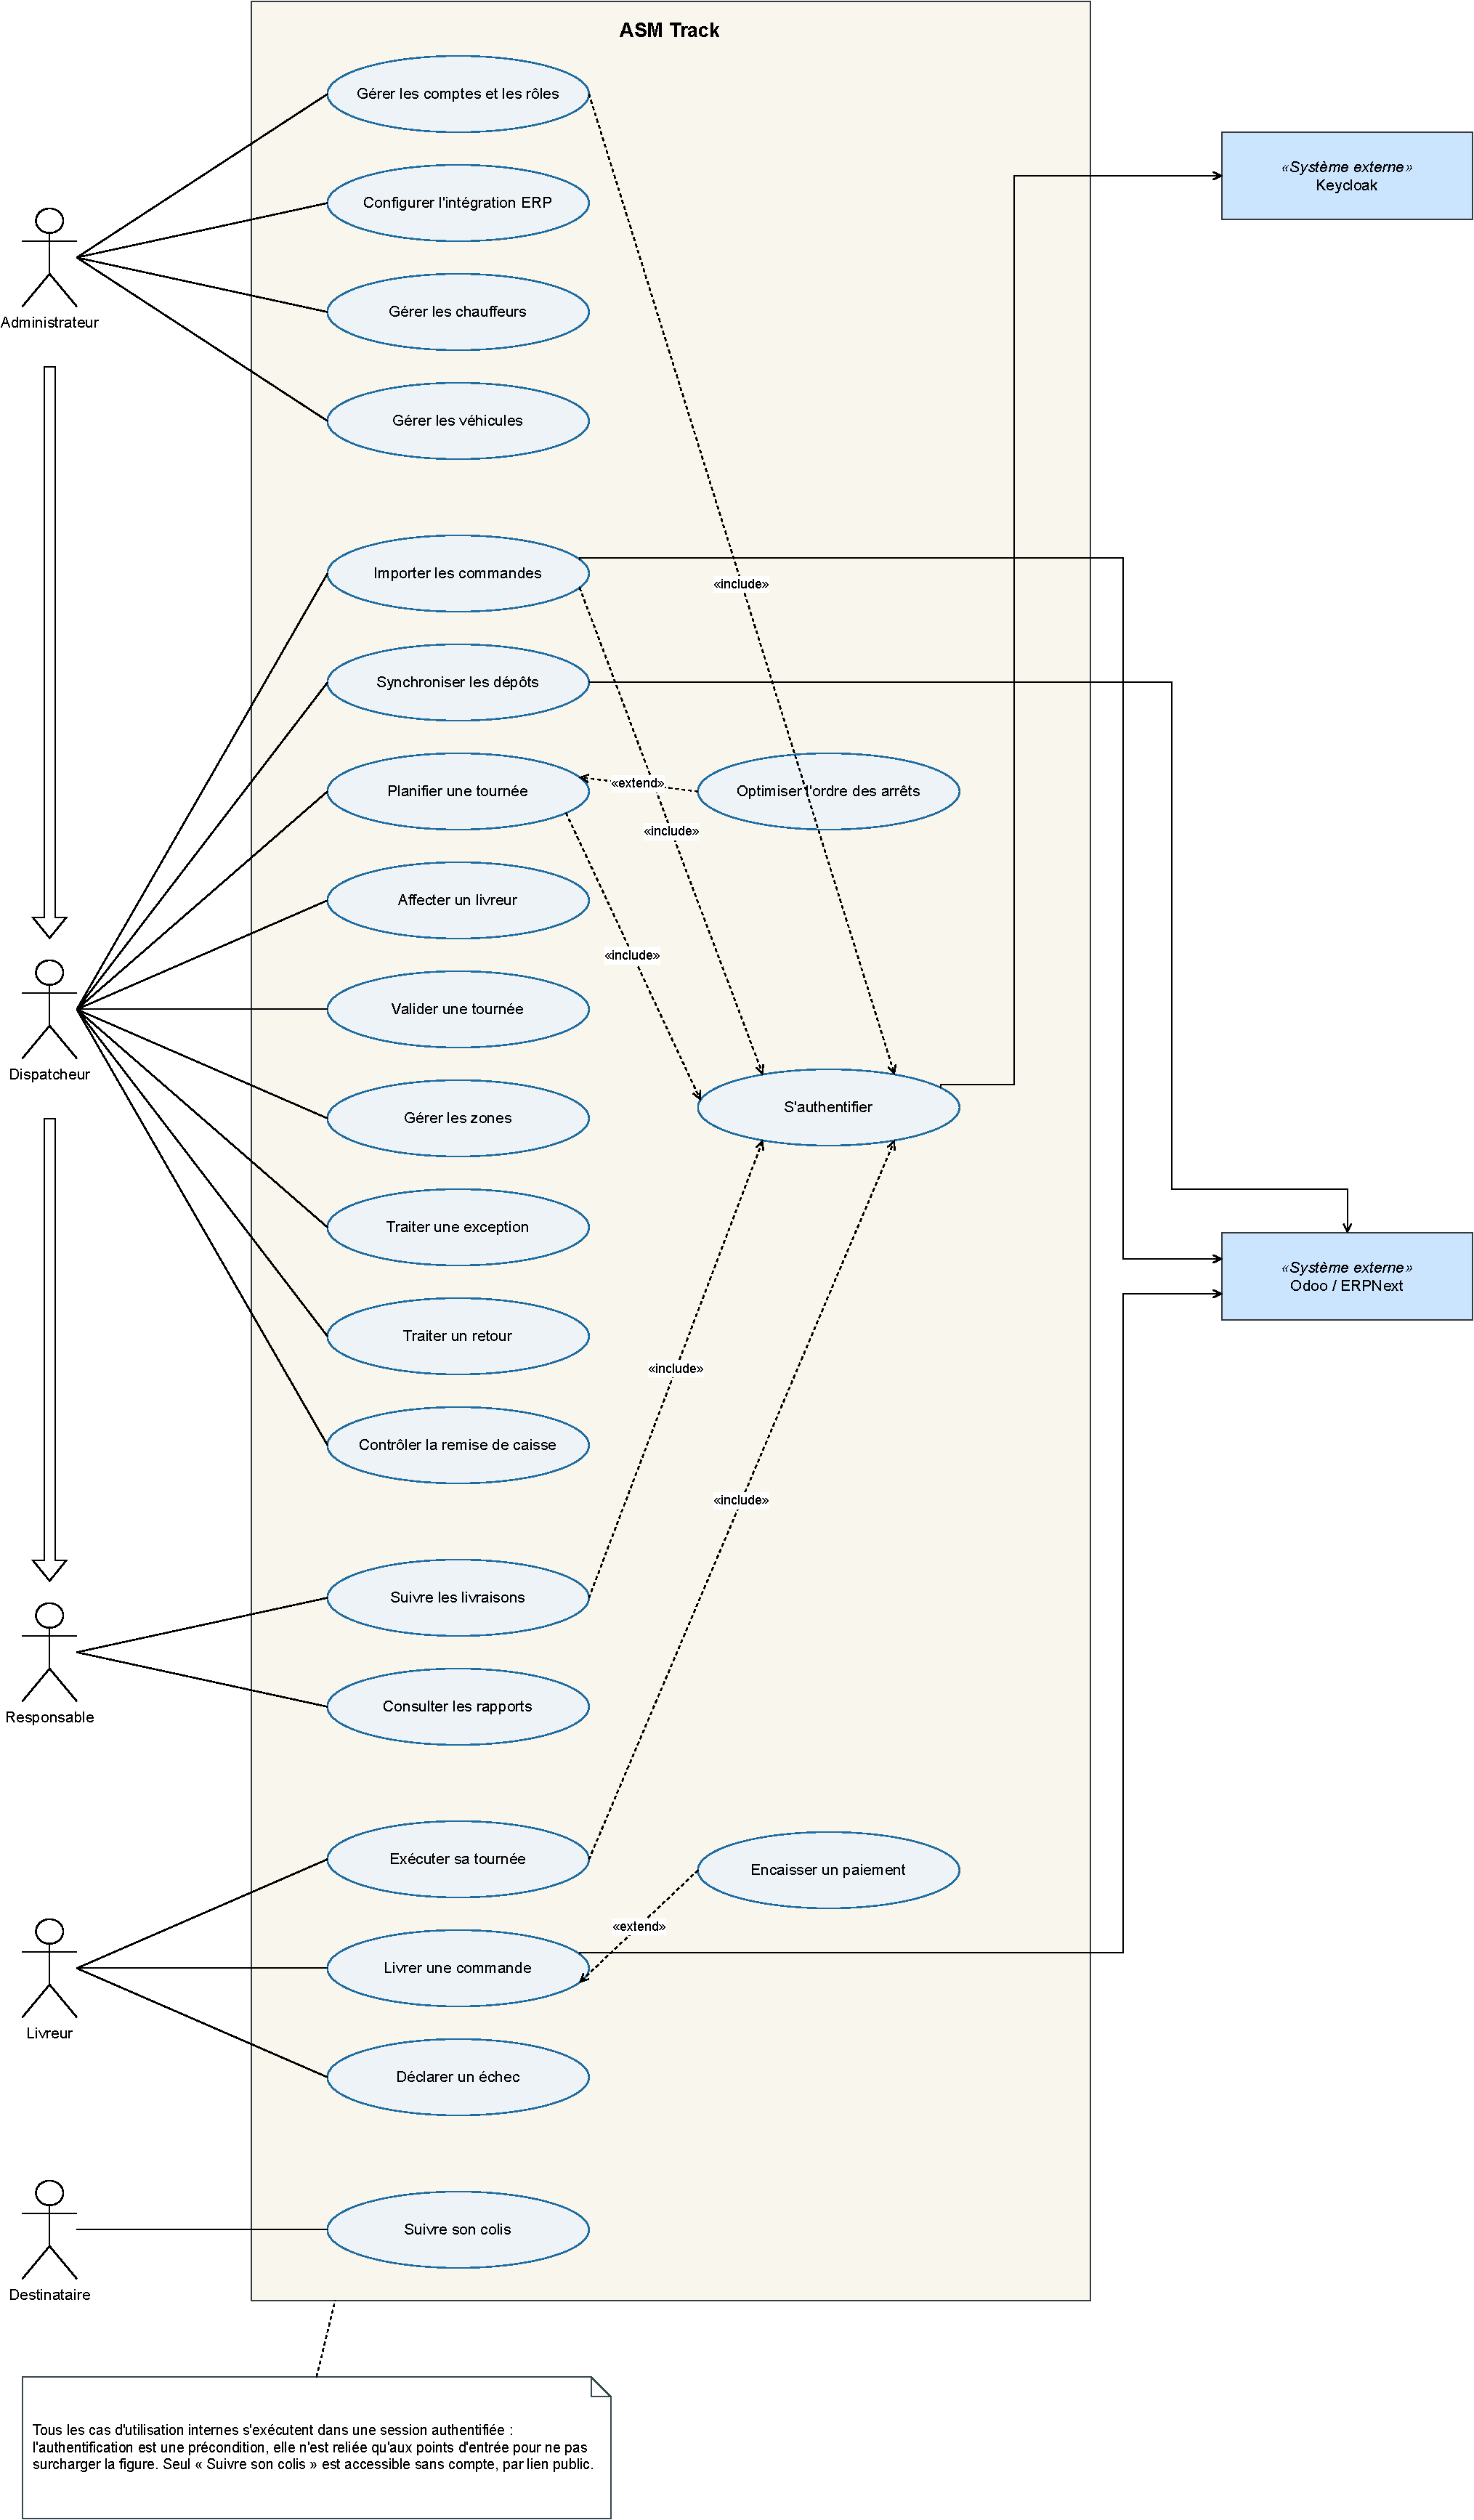
\includegraphics[width=\textwidth,height=0.86\textheight,keepaspectratio]{uc-global}
\caption{Diagramme global des cas d'utilisation}
\label{fig:uc-global}
\end{figure}

Trois éléments de lecture méritent d'être soulignés.

\textbf{Une seule généralisation relie les acteurs}~: l'administrateur est un dispatcheur qui dispose
en plus du paramétrage, et ses permissions incluent effectivement toutes celles du dispatcheur. La
flèche évite de redessiner une douzaine de traits.

Le responsable, lui, reste rattaché à ses propres cas. Il croise le dispatcheur sur les consultations
sans jamais le contenir ni en dériver~: il est seul à accéder au journal d'audit, et n'a aucune des
permissions d'action. Superviser suppose de pouvoir relire ce que font ceux qui opèrent, sans
pouvoir opérer soi-même~; c'est pourquoi les rôles sont déclarés à plat dans l'annuaire, chacun
portant sa liste explicite, plutôt qu'en chaîne d'héritage. Le chapitre~\ref{ch:socle} détaille ce
modèle.

Les liens \emph{«~include~»} vers le cas \emph{S'authentifier} ne sont tracés que depuis les points
d'entrée. L'authentification est en réalité une précondition de tous les cas internes~; la relier à
chacun surchargerait la figure sans rien apprendre au lecteur. Le destinataire, lui, en est
véritablement exempt~: son suivi passe par un lien public et n'exige aucun compte.

Les deux liens \emph{«~extend~»} signalent des cas facultatifs. \emph{Optimiser l'ordre des arrêts}
étend \emph{Planifier une tournée}, parce que le dispatcheur peut toujours ordonner ses arrêts
lui-même. \emph{Encaisser un paiement} étend \emph{Livrer une commande}, parce que toutes les
commandes ne sont pas payables à la livraison.

\subsection{Diagramme de classes global}

Le diagramme de la figure~\ref{fig:class-global} présente les concepts manipulés par le système et
leurs relations. Il fixe le vocabulaire employé dans tout le reste du rapport.

\begin{figure}[H]
\centering
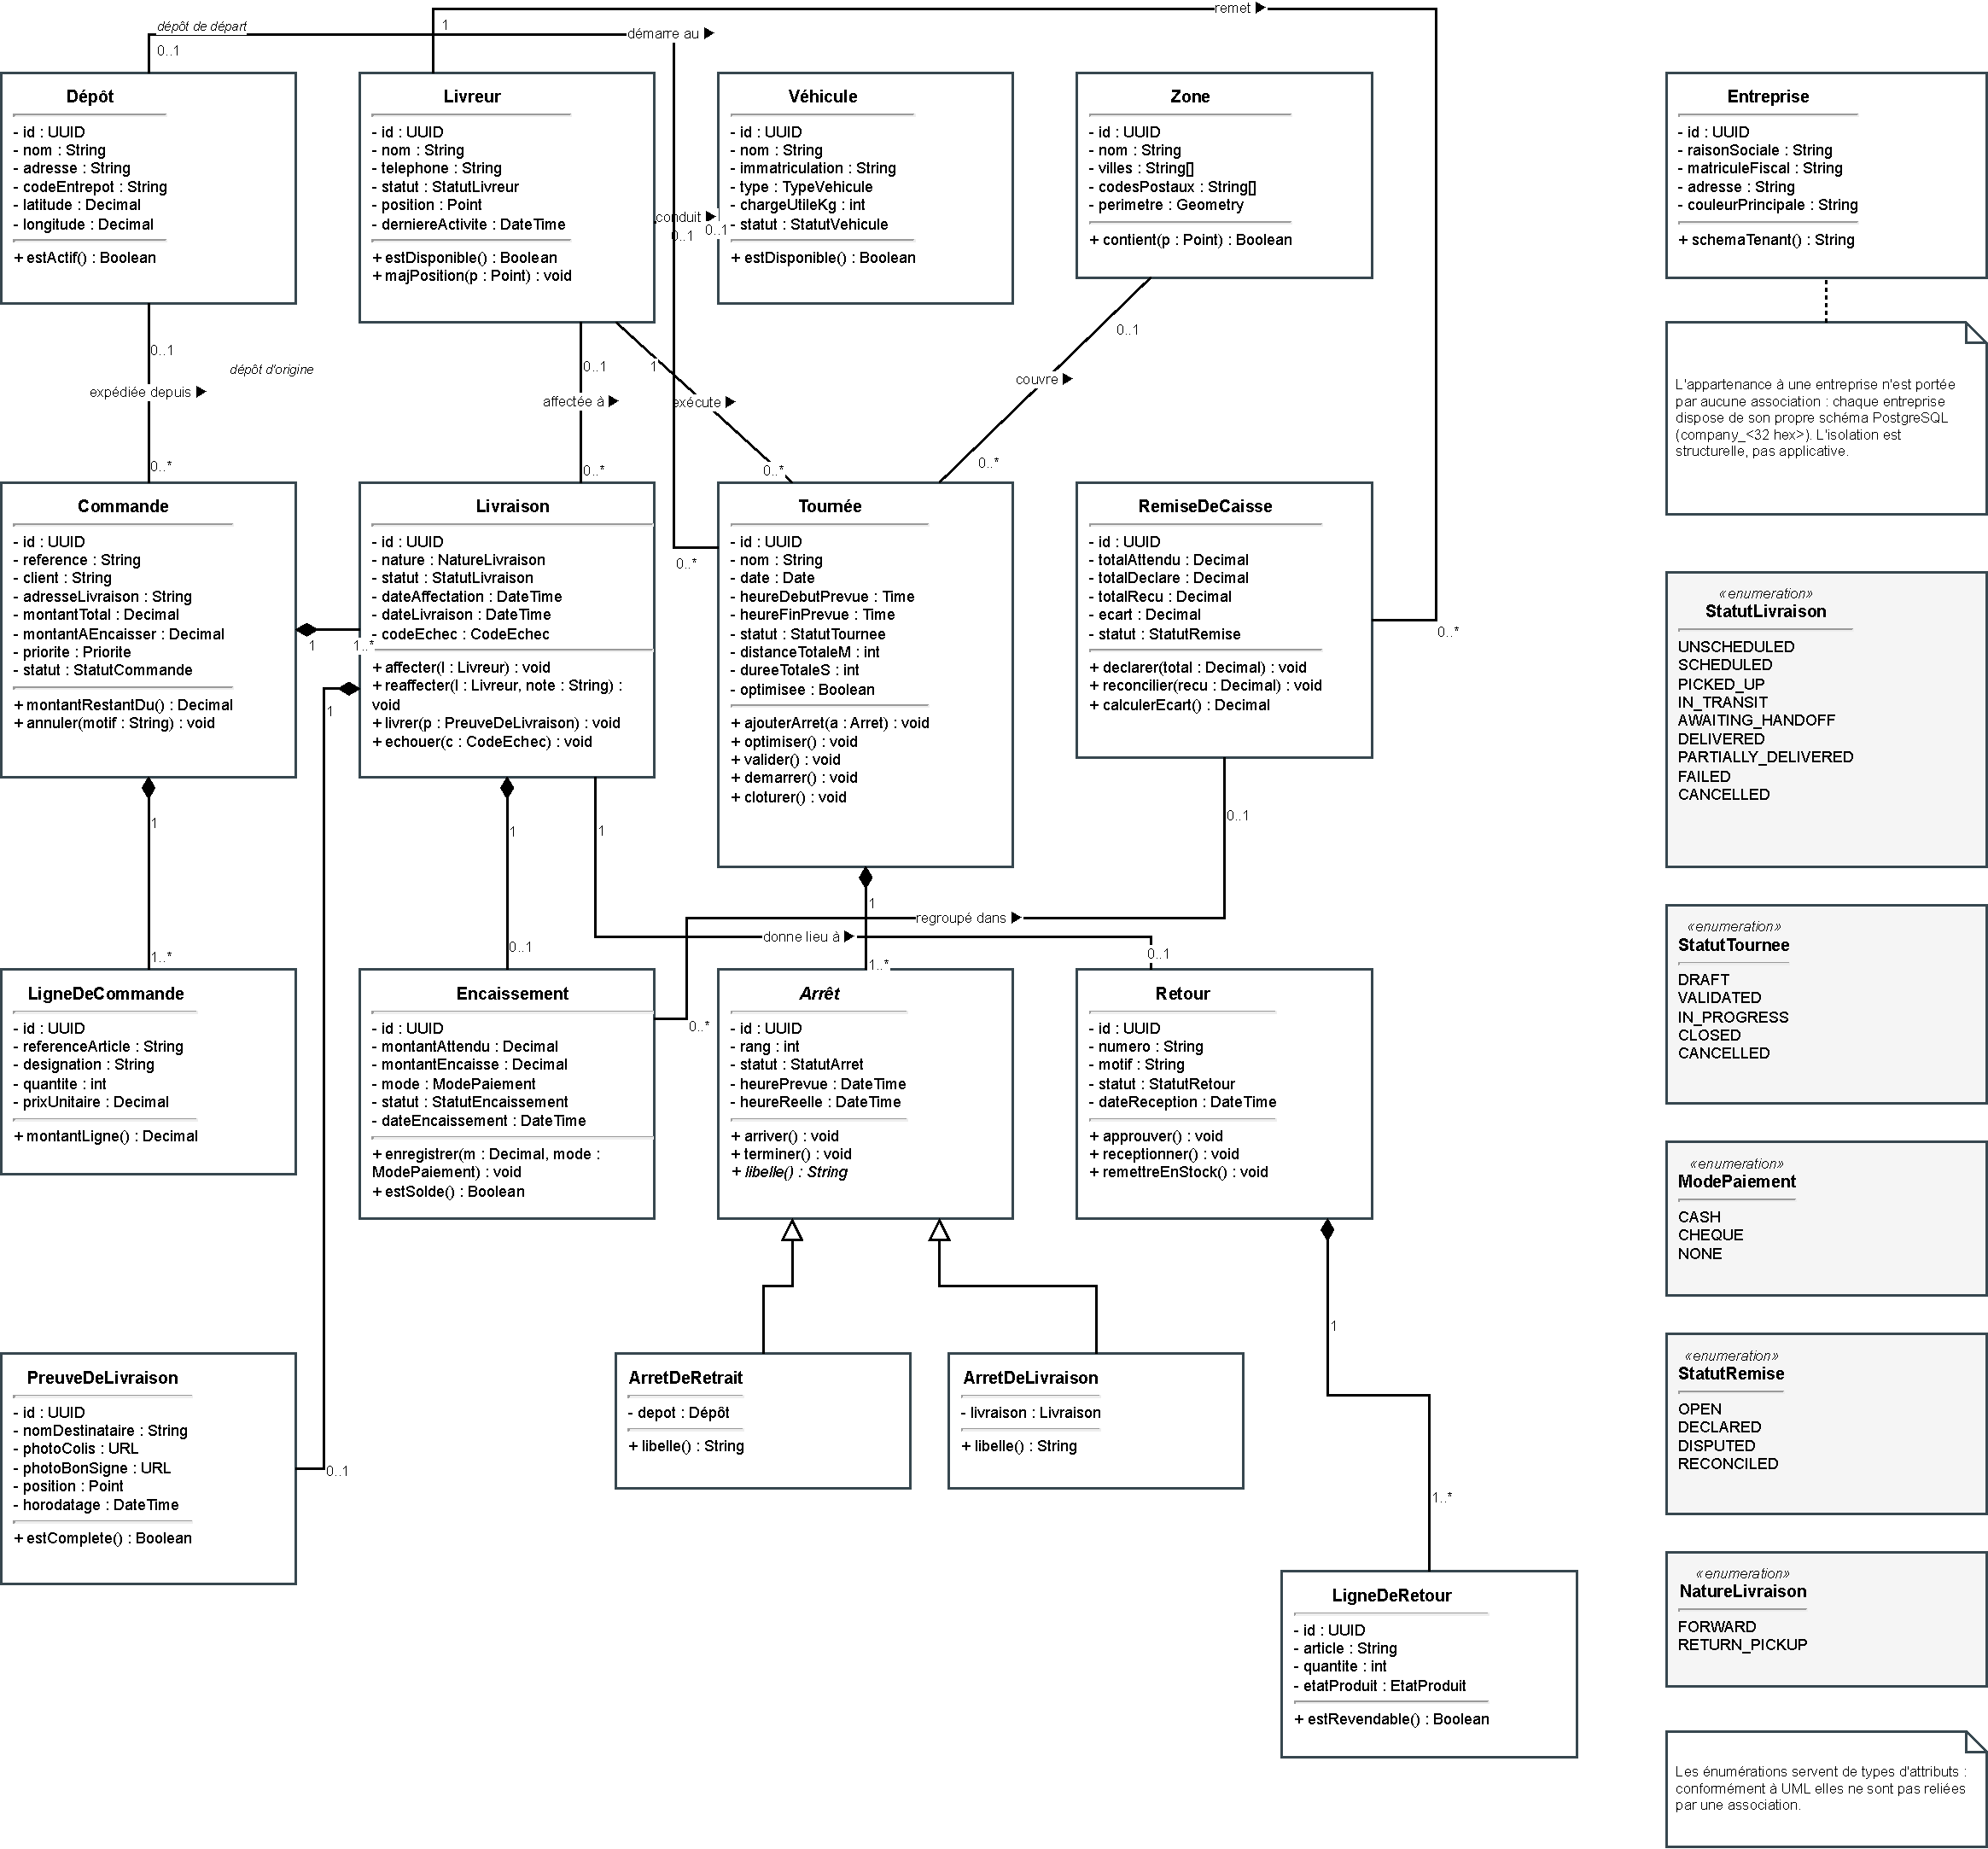
\includegraphics[width=\textwidth,height=0.86\textheight,keepaspectratio]{class-domain}
\caption{Diagramme de classes global}
\label{fig:class-global}
\end{figure}

Il se lit de haut en bas, du référentiel vers l'exécution. La partie haute regroupe ce qui existe
avant toute commande~: dépôts, chauffeurs, véhicules et zones. Au centre, une \textbf{Commande}
issue du progiciel se décompose en une ou plusieurs \textbf{Livraisons}~; le losange plein indique
une composition, c'est-à-dire que les livraisons n'ont pas d'existence propre en dehors de leur
commande. En parallèle, un chauffeur exécute des \textbf{Tournées}, elles-mêmes composées
d'\textbf{Arrêts}.

La classe \emph{Arrêt} est abstraite, et c'est le point le moins évident du modèle. Un arrêt de
retrait désigne un dépôt où le chauffeur charge~; un arrêt de livraison désigne une livraison à
remettre. Ce ne sont pas les mêmes objets, d'où la généralisation~: les représenter par un simple
attribut « type » aurait masqué une différence de structure réelle.

La partie basse porte les traces laissées par l'exécution~: une \textbf{PreuveDeLivraison}, un
\textbf{Encaissement} lorsque le client règle à la porte, et un \textbf{Retour} si la marchandise
revient. Les encaissements d'un chauffeur sont ensuite regroupés dans une \textbf{RemiseDeCaisse},
ce qui matérialise la séparation des responsabilités~: celui qui déclare la somme n'est pas celui
qui la valide.

Enfin, la classe \textbf{Entreprise} n'est reliée à rien, et c'est délibéré. L'appartenance d'une
donnée à une entreprise cliente n'est pas portée par une clé étrangère mais par un schéma de base de
données distinct. Le chapitre~\ref{ch:archi} détaille ce mécanisme.

\section{Gestion du projet avec Scrum}

\subsection{Product Backlog}

Le \emph{product backlog} traduit les besoins fonctionnels en éléments réalisables et priorisés. Ils
ont été formulés sous forme de \emph{user stories}, selon le gabarit « en tant que \emph{rôle}, je
veux \emph{action}, afin de \emph{bénéfice} », puis regroupés en huit épopées correspondant aux
domaines de la section précédente.

Deux échelles complètent chaque élément. La \textbf{priorité} suit la méthode MoSCoW —
\emph{Must~have} pour l'indispensable, \emph{Should~have} pour l'important non bloquant,
\emph{Could~have} pour le souhaitable. L'\textbf{estimation} est exprimée en points de complexité
selon la suite de Fibonacci~; il s'agit d'une complexité relative entre éléments, non d'une durée.

\begin{longtable}{L{1.1cm}L{8.2cm}C{1.5cm}C{1.1cm}C{1.3cm}}
\caption{Product Backlog du projet}
\label{tab:backlog} \\
\hline
\rowcolor{isimsblue!10}
\textbf{Réf.} & \textbf{User story} & \textbf{Priorité} & \textbf{Est.} & \textbf{Sprint} \\
\hline
\endfirsthead
\multicolumn{5}{c}{\tablename\ \thetable{} — \emph{suite}} \\
\hline
\rowcolor{isimsblue!10}
\textbf{Réf.} & \textbf{User story} & \textbf{Priorité} & \textbf{Est.} & \textbf{Sprint} \\
\hline
\endhead
\hline
\multicolumn{5}{r}{\emph{suite page suivante}} \\
\endfoot
\hline
\endlastfoot

\multicolumn{5}{l}{\cellcolor{isimsblue!5}\textbf{Épopée 1 — Identités, autorisations et multi-tenance}} \\
\hline
US-01 & En tant qu'utilisateur, je veux m'authentifier par un compte unique afin d'accéder aux écrans
correspondant à mon rôle. & Must & 8 & 1 \\
\hline
US-02 & En tant qu'administrateur, je veux créer des comptes et leur attribuer un rôle afin de
contrôler qui accède à quoi. & Must & 5 & 1 \\
\hline
US-03 & En tant qu'administrateur, je veux que chaque opération vérifie la permission portée par le
rôle de l'utilisateur afin que personne ne puisse dépasser ses droits. & Must & 8 & 1 \\
\hline
US-04 & En tant qu'entreprise cliente, je veux que mes données soient inaccessibles aux autres
entreprises hébergées afin de garantir ma confidentialité. & Must & 13 & 1 \\
\hline

\multicolumn{5}{l}{\cellcolor{isimsblue!5}\textbf{Épopée 2 — Intégration au progiciel de gestion}} \\
\hline
US-05 & En tant que dispatcheur, je veux importer les commandes prêtes depuis le progiciel afin de ne
pas les ressaisir. & Must & 13 & 2 \\
\hline
US-06 & En tant qu'administrateur, je veux relier les champs de mon progiciel à ceux du système afin
d'adapter l'intégration à mon paramétrage. & Must & 13 & 2 \\
\hline
US-07 & En tant qu'entreprise, je veux pouvoir brancher la solution sur n'importe quel progiciel de
gestion afin de ne dépendre d'aucun éditeur. & Must & 21 & 2 \\
\hline
US-08 & En tant que dispatcheur, je veux que le statut d'une livraison remonte automatiquement dans le
progiciel afin que la facturation suive. & Must & 8 & 2 \\
\hline
US-09 & En tant que dispatcheur, je veux qu'une synchronisation interrompue soit réessayée puis
signalée afin qu'aucune information ne se perde silencieusement. & Must & 13 & 2 \\
\hline
US-10 & En tant que dispatcheur, je veux récupérer les entrepôts du progiciel comme dépôts afin
d'éviter un double référentiel. & Should & 5 & 2 \\
\hline
US-11 & En tant qu'administrateur, je veux que le système fonctionne avec plusieurs versions du même
progiciel afin de ne pas imposer de montée de version au client. & Should & 13 & 2 \\
\hline

\multicolumn{5}{l}{\cellcolor{isimsblue!5}\textbf{Épopée 3 — Référentiel logistique}} \\
\hline
US-12 & En tant qu'administrateur, je veux gérer la liste des chauffeurs afin de refléter l'équipe
réelle. & Must & 5 & 1 \\
\hline
US-13 & En tant qu'administrateur, je veux gérer le parc de véhicules avec leur capacité afin de
pouvoir les affecter. & Should & 5 & 1 \\
\hline
US-14 & En tant qu'administrateur, je veux définir des zones géographiques afin de regrouper les
livraisons par secteur. & Should & 8 & 1 \\
\hline

\multicolumn{5}{l}{\cellcolor{isimsblue!5}\textbf{Épopée 4 — Planification et affectation}} \\
\hline
US-15 & En tant que dispatcheur, je veux construire une tournée à partir de livraisons afin
d'organiser la journée. & Must & 13 & 3 \\
\hline
US-16 & En tant que dispatcheur, je veux affecter un chauffeur et un véhicule à une tournée afin d'en
désigner le responsable. & Must & 8 & 3 \\
\hline
US-17 & En tant que dispatcheur, je veux obtenir un ordre de passage optimisé afin de réduire la
distance parcourue. & Should & 13 & 3 \\
\hline
US-18 & En tant que dispatcheur, je veux valider une tournée afin de la rendre visible au chauffeur.
& Must & 5 & 3 \\
\hline
US-19 & En tant que dispatcheur, je veux connaître l'heure d'arrivée estimée à chaque arrêt afin de
détecter les retards. & Should & 8 & 3 \\
\hline

\multicolumn{5}{l}{\cellcolor{isimsblue!5}\textbf{Épopée 5 — Exécution terrain}} \\
\hline
US-20 & En tant que chauffeur, je veux consulter ma tournée du jour sur mon téléphone afin de savoir
où aller. & Must & 8 & 4 \\
\hline
US-21 & En tant que chauffeur, je veux déclarer une livraison réussie ou échouée avec un motif afin
que le bureau soit informé. & Must & 8 & 4 \\
\hline
US-22 & En tant que chauffeur, je veux enregistrer une preuve de livraison avec photographies afin de
couvrir l'entreprise en cas de litige. & Must & 13 & 4 \\
\hline
US-23 & En tant que chauffeur, je veux continuer à travailler sans réseau et voir mes actions
transmises au retour de la couverture afin de ne jamais être bloqué. & Must & 21 & 4 \\
\hline
US-24 & En tant que chauffeur, je veux transmettre un colis à un collègue avec confirmation afin que
la responsabilité soit tracée. & Should & 13 & 4 \\
\hline

\multicolumn{5}{l}{\cellcolor{isimsblue!5}\textbf{Épopée 6 — Encaissement et remise de caisse}} \\
\hline
US-25 & En tant que chauffeur, je veux enregistrer le montant encaissé et son mode de règlement afin
d'en garder la trace. & Must & 8 & 4 \\
\hline
US-26 & En tant que chauffeur, je veux déclarer le total remis en fin de tournée afin de clore ma
journée. & Must & 5 & 4 \\
\hline
US-27 & En tant que dispatcheur, je veux compter la somme reçue et arbitrer l'écart afin que la
caisse soit vérifiable. & Must & 8 & 4 \\
\hline

\multicolumn{5}{l}{\cellcolor{isimsblue!5}\textbf{Épopée 7 — Suivi, aléas et retours}} \\
\hline
US-28 & En tant que dispatcheur, je veux voir l'avancement des livraisons sans recharger la page afin
de réagir immédiatement. & Must & 13 & 3 \\
\hline
US-29 & En tant que dispatcheur, je veux être alerté des retards et des échecs afin de traiter les
exceptions en priorité. & Must & 8 & 3 \\
\hline
US-30 & En tant que dispatcheur, je veux réaffecter une livraison bloquée à un autre chauffeur afin
de sauver la journée. & Must & 8 & 3 \\
\hline
US-31 & En tant que dispatcheur, je veux approuver ou refuser une demande de retour et déclencher
la reprise en stock afin de garder la main sur ce qui revient. & Should & 8 & 3 \\
\hline
US-32 & En tant que destinataire, je veux suivre mon colis par un lien reçu afin de connaître son
avancement sans créer de compte. & Should & 8 & 3 \\
\hline

\multicolumn{5}{l}{\cellcolor{isimsblue!5}\textbf{Épopée 8 — Pilotage et exploitation}} \\
\hline
US-33 & En tant que responsable, je veux consulter les indicateurs de performance afin de piloter
l'activité. & Should & 13 & 5 \\
\hline
US-34 & En tant que responsable, je veux exporter un rapport de tournée afin de le transmettre ou de
l'archiver. & Should & 8 & 5 \\
\hline
US-35 & En tant qu'administrateur, je veux une console indiquant l'état de l'intégration afin de
distinguer une panne du progiciel d'une panne du système. & Must & 13 & 5 \\
\hline
US-36 & En tant qu'administrateur, je veux relancer une synchronisation en échec afin de réparer sans
intervention technique. & Must & 8 & 5 \\
\hline
US-37 & En tant qu'administrateur, je veux consulter le journal des opérations sensibles afin de
pouvoir répondre à un audit. & Should & 8 & 5 \\
\hline
US-38 & En tant qu'utilisateur, je veux interroger une assistance interne sur le fonctionnement du
système afin de trouver une réponse sans quitter l'application. & Could & 13 & 5 \\
US-39 & En tant que destinataire, je veux demander le retour d'un article reçu afin de ne pas avoir
à téléphoner. & Should & 5 & 3 \
US-40 & En tant que chauffeur, je veux collecter un retour chez le destinataire afin de le ramener
au dépôt. & Should & 5 & 4 \\
\hline
\end{longtable}

Le backlog totalise quarante éléments pour 387 points de complexité. Il a été tenu dans
\textbf{GitLab Issues}, chaque épopée correspondant à une étiquette et chaque sprint à un tableau
kanban dédié.

\subsection{Planification des sprints}

Le projet s'est déroulé du 2~mars au 17~août 2026, soit vingt-quatre semaines. Il a été découpé en un
sprint d'initialisation et cinq sprints fonctionnels de trois à cinq semaines, chacun clos par une
revue et une rétrospective avant l'engagement du suivant.

L'ordre des sprints obéit à une contrainte simple~: chaque sprint ne doit dépendre que de ce qui a
déjà été livré. L'isolation par entreprise et le contrôle des droits viennent en premier, parce que
toute donnée créée ensuite doit déjà être rattachée à un client et protégée — les rajouter après coup
aurait imposé de reprendre l'ensemble du code écrit entre-temps. L'intégration au progiciel vient
juste après, parce qu'elle alimente le système en commandes~: sans elle, les sprints suivants
auraient travaillé sur des données saisies à la main, donc sur un cas qui n'existe pas en
production.

\begin{table}[H]
\centering
\caption{Planification des sprints}
\label{tab:planning}
% Colonne « Objectif » élargie et intitulés raccourcis pour qu'aucune ligne ne passe sur deux
% lignes : le tableau tient alors dans la place laissée par le texte au lieu d'être repoussé.
\small
\begin{tabular}{L{1.5cm}L{5.6cm}C{3.2cm}C{1.5cm}C{1.4cm}}
\hline
\rowcolor{isimsblue!10}
\textbf{Sprint} & \textbf{Objectif} & \textbf{Période} & \textbf{Durée} & \textbf{Points} \\
\hline
Sprint 0 & Cadrage, besoins et étude technique & 2 — 20 mars & 3 sem. & — \\
\hline
Sprint 1 & Identité, autorisation et multi-tenance & 23 mars — 17 avril & 4 sem. & 34 \\
\hline
Sprint 2 & Intégration ERP agnostique & 20 avril — 22 mai & 5 sem. & 86 \\
\hline
Sprint 3 & Planification et suivi temps réel & 25 mai — 19 juin & 4 sem. & 115 \\
\hline
Sprint 4 & Application chauffeur et hors ligne & 22 juin — 17 juillet & 4 sem. & 84 \\
\hline
Sprint 5 & Exploitation, résilience et assistance & 20 juillet — 7 août & 3 sem. & 63 \\
\hline
\multicolumn{2}{l}{Recette, rédaction et soutenance} & 10 — 17 août & 1 sem. & — \\
\hline
\end{tabular}
\end{table}

Les sprints~2 et~3 concentrent à eux seuls plus de la moitié des points. Le premier parce que
l'indépendance vis-à-vis du progiciel exige une couche d'abstraction complète avant le moindre gain
visible~; le second parce qu'il porte le cœur métier de la solution.

\section{Étude technique}

\subsection{Environnement matériel}

Le développement a été mené sur un poste unique, qui a également hébergé l'ensemble des services
conteneurisés — bases de données, courtier de messages, serveur d'identité, moteur de calcul
d'itinéraires et instances de progiciel de test. Cette dernière contrainte explique le
dimensionnement en mémoire.

\begin{table}[H]
\centering
\caption{Environnement matériel de développement}
\label{tab:materiel}
\begin{tabular}{L{4.5cm}L{10cm}}
\hline
\rowcolor{isimsblue!10}
\textbf{Élément} & \textbf{Caractéristique} \\
\hline
Processeur & Intel Core i5-12450H, 12\textsuperscript{e} génération \\
\hline
Mémoire vive & 24 Go \\
\hline
Système d'exploitation & Windows 11 Professionnel \\
\hline
Exécution des services & Docker Desktop, moteur WSL~2 \\
\hline
Essais mobiles & Appareil Android physique et émulateur \\
\hline
\end{tabular}
\end{table}

\subsection{Environnement logiciel de développement}

\begin{table}[H]
\centering
\caption{Outils de développement et de collaboration}
\label{tab:outils}
\begin{tabular}{L{4.5cm}L{10cm}}
\hline
\rowcolor{isimsblue!10}
\textbf{Outil} & \textbf{Usage dans le projet} \\
\hline
Visual Studio Code & Éditeur principal pour le code Java, TypeScript et Dart \\
\hline
Android Studio & Compilation, émulation et débogage de l'application chauffeur \\
\hline
Git et GitLab & Gestion de versions, suivi du backlog par issues et tableaux, intégration continue \\
\hline
Docker Desktop & Exécution locale de l'ensemble des services et de leurs dépendances \\
\hline
Postman & Essais manuels des interfaces de programmation \\
\hline
DBeaver & Inspection des schémas et des données PostgreSQL \\
\hline
draw.io & Conception des diagrammes UML du présent rapport \\
\hline
\LaTeX{} (XeLaTeX) & Rédaction du rapport \\
\hline
\end{tabular}
\end{table}

\subsection{Technologies retenues}

Le choix des technologies a été arrêté au terme du sprint~0, chaque brique étant retenue pour une
raison rattachable à un besoin de la section~\ref{sec:besoins}. Le chapitre~\ref{ch:archi} en détaille
la mise en œuvre.

\begin{table}[H]
\centering
\caption{Technologies retenues et motif du choix}
\label{tab:technos}
\begin{tabular}{L{2.5cm}L{3.4cm}L{8.6cm}}
\hline
\rowcolor{isimsblue!10}
\textbf{Couche} & \textbf{Technologie} & \textbf{Motif du choix} \\
\hline
Services & Spring Boot 3.3.5, Java 17 & Écosystème mature pour les architectures en services, avec
prise en charge native de la sécurité par jetons et du multi-schéma \\
\hline
Passerelle & Spring Cloud Gateway & Point d'entrée unique~: validation des jetons et application des
droits avant tout accès aux services \\
\hline
Interface web & React 19, Vite, TypeScript & Rendu réactif adapté à un tableau de dispatch qui se met
à jour en continu \\
\hline
Application mobile & Flutter & Base de code unique, et stockage local performant sur lequel repose le
mode hors ligne \\
\hline
Base de données & PostgreSQL 16 & Schéma par entreprise cliente pour l'isolation, type
\texttt{jsonb} pour les données de forme variable, absence de coût de licence \\
\hline
Messagerie & RabbitMQ 4 & Découplage des échanges avec le progiciel, relances et file de rebut
intégrées \\
\hline
Identité & Keycloak & Serveur OpenID Connect éprouvé, gestion native des organisations \\
\hline
Fichiers & MinIO & Stockage compatible S3 des photographies de preuve, déployable localement \\
\hline
Itinéraires & OSRM & Moteur de calcul auto-hébergé, sans coût par requête ni dépendance à un service
externe \\
\hline
\end{tabular}
\end{table}

\paragraph*{Sur le choix de la base de données.} PostgreSQL a été retenu pour deux raisons directement
liées aux besoins structurants. La première est l'isolation par entreprise cliente~: PostgreSQL
permet de créer un schéma par client au sein d'une même base et d'en changer dynamiquement à chaque
requête, mécanisme sur lequel repose toute la multi-tenance décrite au chapitre~\ref{ch:archi}. La
seconde est le stockage semi-structuré~: le détail des lignes de commande et les champs
supplémentaires propres à chaque client varient d'un progiciel à l'autre, ce que le type
\texttt{jsonb} absorbe sans multiplier les tables. S'y ajoute l'absence de coût de licence, cohérente avec une solution
destinée à être déployée chez plusieurs clients.

\section{Conclusion}

Ce sprint d'initialisation a produit quatre livrables~: la liste des acteurs et de leurs droits, la
spécification des besoins fonctionnels et non fonctionnels, les deux diagrammes qui fixent le
vocabulaire du système, et un backlog de quarante éléments réparti sur cinq sprints.

Son apport principal n'est pourtant pas cette production documentaire. Il tient à trois exigences que
l'analyse a fait remonter au rang de contraintes structurantes~: l'ouverture à plusieurs progiciels,
l'hébergement de plusieurs entreprises clientes sur une même installation, et la continuité de
service en l'absence de réseau. Aucune n'est une fonctionnalité visible pour l'utilisateur, et
pourtant toutes trois ont déterminé l'architecture, l'ordre des sprints et une partie des choix
technologiques.

Le chapitre suivant présente cette architecture. Les cinq chapitres qui lui succèdent déroulent
ensuite les sprints dans l'ordre du tableau~\ref{tab:planning}.

% Budget : 13 pages — voir rapport/PLAN.md
\chapter{Architecture et conception générale}
\label{ch:archi}

\section{Introduction}

\section{Conclusion}

% Budget : 15 pages — voir rapport/PLAN.md
\chapter{Sprint 1 — Socle d'identité, d'autorisation et de multi-tenance}
\label{ch:socle}

\section{Introduction}

\section{Conclusion}

% Budget : 16 pages — voir rapport/PLAN.md
\chapter{Sprint 2 — Intégration ERP agnostique}
\label{ch:erp}

\section{Introduction}

\section{Conclusion}

% Budget : 14 pages — voir rapport/PLAN.md
\chapter{Sprint 3 — Planification, exécution et suivi temps réel}

\section{Introduction}

\section{Conclusion}

% Budget : 12 pages — voir rapport/PLAN.md
\chapter{Sprint 4 — Application mobile chauffeur et mode hors ligne}

\section{Introduction}

\section{Conclusion}

% Budget : 11 pages — voir rapport/PLAN.md
\chapter{Sprint 5 — Exploitation, résilience et assistant interne}
\label{ch:ops}

\section{Introduction}

\section{Conclusion}

% Budget : 9 pages — voir rapport/PLAN.md
\chapter{Validation globale, qualité et déploiement}
\label{ch:validation}

\section{Introduction}

\section{Conclusion}

\chapter*{Conclusion générale et perspectives}
\addcontentsline{toc}{chapter}{Conclusion générale et perspectives}
\markboth{CONCLUSION GÉNÉRALE}{}

% Budget : 3 pages.
\clearpage


% ---------- Bibliographie et annexes ----------
% Le guide de l'institut demande une bibliographie et une webographie distinctes : les ouvrages,
% articles et actes d'un côté, la documentation en ligne des solutions étudiées de l'autre.
\printbibliography[heading=bibintoc,title={Bibliographie},nottype=online]
\printbibliography[heading=bibintoc,title={Webographie},type=online]

\appendix
\chapter{Annexes}


% Quatrième de couverture imposée par l'institut : résumé arabe, français et anglais. Elle ferme le
% mémoire — ce n'est pas une page liminaire.
% =====================================================================
%  Quatrième de couverture — page imposée par le modèle ISIMS.
%  Ordre du modèle : الخلاصة, puis Résumé, puis Abstract, puis les mots clés dans les trois langues.
%
%  Cette page exige XeLaTeX (voir preamble.tex) : l'arabe ne se compose pas sous pdfLaTeX.
% =====================================================================
\clearpage
\thispagestyle{empty}
% Comme la couverture, cette page est imposée et doit tenir sur une seule feuille : avec
% l'interligne 1,5 du corps, les trois résumés et le pied de page débordaient.
\singlespacing

\begin{center}
  {\bfseries\large Système intelligent de suivi de livraison}
\end{center}
\vspace{-0.2cm}
\noindent\textcolor{isimsblue}{\rule{\textwidth}{1pt}}

\begin{center}
  {\Large\bfseries\itshape Mohamed Aziz Hadjkacem}
\end{center}
\vspace{-0.2cm}
\noindent\textcolor{isimsblue}{\rule{\textwidth}{1pt}}

\vspace{0.3cm}
% Le guide de rédaction plafonne chaque résumé à 10 lignes (règle 6) : à ce format, en corps 12
% normal, les trois versions ci-dessous tiennent sans avoir besoin de réduire la police.

% --- Arabe -----------------------------------------------------------------
% Le titre est aligné à droite et le paragraphe composé de droite à gauche : dans le modèle, tout le
% bloc arabe est en RTL, y compris la ponctuation finale.
\begin{Arabic}
\begin{flushright}
\textbf{\underline{الخلاصة}} : تقدّم هذه المذكّرة منصّة لتتبّع عمليات التوصيل في الكيلومتر الأخير،
قابلة للاستعمال من قِبَل عدّة مؤسسات ومندمجة مع أنظمة تخطيط مواردها. تغطّي المنصّة استيراد الطلبات
من نظام تخطيط الموارد، وتخطيط الجولات، والتنفيذ الميداني عبر تطبيق جوّال يعمل دون اتصال بالإنترنت،
وإثبات التسليم، وإدارة الإرجاع. تعتمد البنية على الخدمات المصغّرة مع عزل البيانات حسب المخطّط،
ومصادقة مفوّضة عبر OAuth2/OIDC، ومُهايئ محايد لأنظمة تخطيط الموارد تم التحقّق منه على Odoo
وERPNext. تمّت النمذجة باستخدام UML وفق منهجية Scrum.
\end{flushright}
\end{Arabic}

\vspace{0.15cm}

% --- Français --------------------------------------------------------------
\noindent\textbf{\underline{Résumé}} : Ce mémoire présente une plateforme de suivi de livraison du
dernier kilomètre, exploitable par plusieurs entreprises clientes et intégrée à leurs progiciels de
gestion. Elle couvre l'import des commandes depuis l'ERP, la planification des tournées, l'exécution
sur le terrain via une application mobile fonctionnant hors connexion, la preuve de livraison et la
gestion des retours. L'architecture, orientée microservices, isole les données par schéma, délègue
l'authentification en OAuth2/OIDC et intègre un adaptateur ERP agnostique validé sur Odoo et
ERPNext. La modélisation a été réalisée en UML et le développement conduit selon la méthode Scrum.

\vspace{0.15cm}

% --- Anglais ---------------------------------------------------------------
\noindent\textbf{\underline{Abstract}}: This thesis presents a last-mile delivery tracking platform,
usable by several client companies and integrated with their enterprise resource planning systems.
It covers order import from the ERP, route planning, field execution through an offline-capable
mobile application, proof of delivery and returns management. The microservice-oriented architecture
isolates data by schema, delegates authentication to OAuth2/OIDC, and integrates an ERP-agnostic
adapter validated against both Odoo and ERPNext. Conceptual modelling was carried out using UML and
development followed the Scrum agile method.

\vspace{0.15cm}

\begin{Arabic}
\begin{flushright}
\textbf{\underline{الكلمات المفاتيح}} : التوصيل في الكيلومتر الأخير، التتبّع الآني، تعدّد
المستأجرين، تكامل أنظمة تخطيط الموارد، الخدمات المصغّرة، العمل دون اتصال، UML.
\end{flushright}
\end{Arabic}

\vspace{0.15cm}

\noindent\textbf{Mots clés} : livraison du dernier kilomètre, suivi en temps réel, multi-tenance,
intégration ERP, Odoo, ERPNext, microservices, mode hors ligne, UML.

\vspace{0.15cm}

\noindent\textbf{Keywords}: last-mile delivery, real-time tracking, multi-tenancy, ERP integration,
Odoo, ERPNext, microservices, offline mode, UML.

% \vfill poussait le pied de page tout en bas de la page disponible et ne lui laissait plus la
% place de s'y tenir : TeX le renvoyait alors, seul, sur une seconde feuille par ailleurs vide.
\vspace{0.5cm}

% --- Pied de page institutionnel (repris du modèle) ---
\noindent\textcolor{isimsblue}{\rule{\textwidth}{0.8pt}}\\[4pt]
\noindent
\begin{minipage}[c]{0.36\textwidth}
  \footnotesize
  www.isimsf.rnu.tn~\raisebox{-2pt}{
\includegraphics[height=10pt]{ico-globe}}\\[4pt]
  % Coupure imposée : laissée au fil du texte, l'adresse cassait après « route de » et rejetait
  % l'icône seule sur une troisième ligne.
  Pôle technologique de Sfax\\
  route de Tunis km 10, B.P. 242 - 3021 Sfax~\raisebox{-2pt}{
\includegraphics[height=10pt]{ico-pin}}
\end{minipage}
\hfill
\begin{minipage}[c]{0.20\textwidth}
  \centering
  
\includegraphics[width=0.9\linewidth]{isims-logo-pied}
\end{minipage}
\hfill
\begin{minipage}[c]{0.30\textwidth}
  \raggedleft\footnotesize
  +216 74 862 432~\raisebox{-2pt}{
\includegraphics[height=10pt]{ico-tel}}\\[4pt]
  +216 74 862 233~\raisebox{-2pt}{
\includegraphics[height=10pt]{ico-fax}}
\end{minipage}


\end{document}
